\documentclass[twoside,a4paper,11pt,openany]{memoir}
\usepackage{a4}
\usepackage{times}
\usepackage{pslatex}
\usepackage{url}
\usepackage{amsmath,amsfonts,amssymb}
\usepackage{mscthesis}
\usepackage{lipsum} % standard filler text, only needed for demo
\usepackage{tikz,pgffor}
\usepackage{minted}
\usepackage{pifont}
\usepackage{multirow}
\usepackage{multicol}
\usetikzlibrary{positioning,shapes.arrows,arrows.meta,shadows,backgrounds,fit}

\usepackage{caption}
% Table float box with bottom caption, box width adjusted to content

%\usepackage[ruled,vlined,linesnumbered]{algorithm2e}
% %% The package 'algorithm' is useful, but incompatible with memoir.
% %% Cor-Paul Bezemer / http://homes.esat.kuleuven.be/~dvherten/esatthesis.html
% %% suggest the following fix:
%\let\newfloat\undefined \usepackage{algorithmic} 
%\usepackage{algorithm}

% Include right (LaTeX/PDFLaTeX) graphics package
% (doesn't work under cygwin apperently)
%\ifx\pdftexversion\undefined
%\usepackage[dvips]{graphicx}
%\usepackage[dvips]{color}
%\usepackage{xcolor,pifont}

%\usepackage[dvipsnames]{xcolor}
\colorlet{gray1}{gray!40!black}
\colorlet{gray2}{gray!80!black}
\usepackage{listings}
\usepackage{subfigure}

\tikzset{XOR/.style={draw,circle,append after command={
        [shorten >=\pgflinewidth, shorten <=\pgflinewidth,]
        (\tikzlastnode.north) edge (\tikzlastnode.south)
        (\tikzlastnode.east) edge (\tikzlastnode.west)
        }
    }
}
\tikzset{line/.style={draw, -latex',shorten <=1bp,shorten >=1bp}}

\lstdefinelanguage{Kotlin}{
  comment=[l]{//},
  commentstyle={\color{gray}\ttfamily},
  emph={filter, first, firstOrNull, forEach, lazy, map, mapNotNull, println},
  emphstyle={\color{OrangeRed}},
  identifierstyle=\color{black},
  keywords={!in, !is, abstract, actual, annotation, as, as?, break, by, catch, class, companion, const, constructor, continue, crossinline, data, delegate, do, dynamic, else, enum, expect, external, false, field, file, final, finally, for, fun, get, if, import, in, infix, init, inline, inner, interface, internal, is, lateinit, noinline, null, object, open, operator, out, override, package, param, private, property, protected, public, receiveris, reified, return, return@, sealed, set, setparam, super, suspend, tailrec, this, throw, true, try, typealias, typeof, val, var, vararg, when, where, while},
  keywordstyle={\color{NavyBlue}\bfseries},
  morecomment=[s]{/*}{*/},
  morestring=[b]",
  morestring=[s]{"""*}{*"""},
  ndkeywords={@Deprecated, @JvmField, @JvmName, @JvmOverloads, @JvmStatic, @JvmSynthetic, Array, Byte, Double, Float, Int, Integer, Iterable, Long, Runnable, Short, String, Any, Unit, Nothing},
  ndkeywordstyle={\color{BurntOrange}\bfseries},
  sensitive=true,
  stringstyle={\color{ForestGreen}\ttfamily},
}


% Colors
% Corporate colors
\definecolor{tudCyan}{RGB}{61,152,222}
\definecolor{tudBlack}{RGB}{0,0,0}
\definecolor{tudWhite}{RGB}{255,255,255}
\definecolor{BurntOrange}{RGB}{204,85,0}
\definecolor{NavyBlue}{RGB}{0,0,128}

% Basic colors
\definecolor{tudSeaGreen}{RGB}{111,189,165}
\definecolor{tudGreen}{RGB}{39,131,142}
\definecolor{tudDarkBlue}{RGB}{34,70,122}
\definecolor{tudPurple}{RGB}{36,46,131}
\definecolor{tudTurquoise}{RGB}{50,154,179}
\definecolor{tudSkyBlue}{RGB}{130,187,206}

% Accent colors
\definecolor{tudLavender}{RGB}{121,150,180}
\definecolor{tudOrange}{RGB}{216,130,62}
\definecolor{tudWarmPurple}{RGB}{110,50,122}
\definecolor{tudFuchsia}{RGB}{178,72,146}
\definecolor{tudBrightGreen}{RGB}{183,200,34}
\definecolor{tudYellow}{RGB}{247,234,151}

\definecolor{customBlockColor}{RGB}{200,228,250}
\definecolor{customAlertColor}{RGB}{31,112,173}

\definecolor{myblue}{rgb}{0.29,0.5,0.74}
\definecolor{myred}{rgb}{0.73,0.32,0.3}
\definecolor{mygreen}{rgb}{0.59,0.73,0.34}
\definecolor{myviolet}{rgb}{0.49,0.39,0.62}
\definecolor{myturquoise}{rgb}{0.28,0.67,0.76}
\definecolor{myorange}{rgb}{0.97,0.58,0.27}
\usepackage{chngcntr}
\counterwithin{figure}{chapter}

\usepackage{parskip}
\setlength{\parskip}{0pt}
%\else
%\usepackage[pdftex]{graphicx}
%\usepackage[pdftex]{color}
%\fi

\usepackage[ruled,vlined,linesnumbered]{algorithm2e}
\usepackage[acronym]{glossaries}
\makeglossaries
\setglossarysection{chapter}

% Used in the bibliography to enable \citeauthor{citation}
\usepackage[numbers]{natbib}
\newcommand*\DNA{\textsc{dna}}

\newcommand*\Let[2]{#1 $\leftarrow$ #2}

% Ensure that urls longer than the page width are broken up
% Based on the answer of StackOverflow user "xamde":
% https://tex.stackexchange.com/a/10401/155506
\expandafter\def\expandafter\UrlBreaks\expandafter{\UrlBreaks%  save the current one
  \do\a\do\b\do\c\do\d\do\e\do\f\do\g\do\h\do\i\do\j%
  \do\k\do\l\do\m\do\n\do\o\do\p\do\q\do\r\do\s\do\t%
  \do\u\do\v\do\w\do\x\do\y\do\z\do\A\do\B\do\C\do\D%
  \do\E\do\F\do\G\do\H\do\I\do\J\do\K\do\L\do\M\do\N%
  \do\O\do\P\do\Q\do\R\do\S\do\T\do\U\do\V\do\W\do\X%
  \do\Y\do\Z}
  

%---------------------------------------------------------------------%
%                     Options                                         %    
%---------------------------------------------------------------------%

\title{Test Program-Based Generative\\ Fuzzing for Differential Testing \\of the Kotlin Compiler}
\subtitle{Version of \today}
% The final version of your thesis should typically use a different
% subtitle without the current date, for example
%\subtitle{Master's Thesis} 
% or remove the subtitle by uncommenting the following line: 
%\subtitle{}

\author{C\u alin-Andrei Georgescu}                               % CHANGE TO YOUR NAME
\authoremail{\url{caling@protonmail.com}}       % CHANGE TO YOUR EMAIL ADDRESS
\birthplace{Bucharest, Romania}                % CHANGE TO YOUR BIRTH PLACE
\studentid{4794672}                              % CHANGE TO YOUR STUDENT ID

% Optional for work done at a company, put this in comments if you did
% not do your thesis work at a company
\company{
%
\includegraphics[height=2cm]{img/hilbert.ps}\\
JetBrains N.V.\\
Huidekoperstraat 26-28\\
1017 ZM Amsterdam, The Netherlands\\
\url{https://www.jetbrains.com/}
}

% Optional (postscript) cover picture. Put this in comments when not needed.
% \coverpicture{
\includegraphics[width=13cm]{img/maze.ps}}


% A copyright notice and maybe something about the cover picture
% Put in comments to get the default copyright notice
%\colophon{\noindent
%  \copyright{} \the\year \: \theauthor. \emph{Note that this notice is for demonstration
%  purposes and that the \LaTeX{} style and document source are free to
%  use as basis for your MSc thesis.} \\[1em] 
%  Cover picture: A ``random'' maze generated in postscript.
%}

% thesis committee:
\chair{Prof. Dr. A. van Deursen, Faculty EEMCS, TU Delft}
\supervisor{Dr. E. Visser, Faculty EEMCS, TU Delft}
% The following two are optional for LaTeX (current university
% regulations state that at least one of them should be assigned)
\externalsupervisor{Drs. E.X. Ternal, Some Company}
\committeemember{Dr. S.T.A.F.F. Member, Faculty EEMCS, TU Delft}


\setcounter{tocdepth}{1}
\setsecnumdepth{subsection}
\maxsecnumdepth{subsection}


\usepackage{hyperref}
\usepackage{cleveref}
\begin{document}
\frontmatter
\thispagestyle{empty}
\maketitle                                      % for the cover page
\makeformaltitlepages{This document describes the standard thesis style for the Software
Engineering department at Delft University of Technology. The document
and it's source are an example of the use of the standard \LaTeX{} style
file. In addition the final appendix to this document contains a
number of requirements and guidelines for writing a Software
Engineering MSc thesis.

Your thesis should either employ this style or follow it closely.


}         % for formal title pages with all info

%\chapter{\label{cha:Preface}Preface}

This is where you thank people for helping you etc.

\lipsum{2} % add some pseudo content

\vskip1cm
\begin{flushright}
\theauthor\\
Delft, the Netherlands \\
\today\\
\end{flushright}



\cleardoublepage\tableofcontents
\cleardoublepage\listoffigures
\cleardoublepage\mainmatter
\addcontentsline{toc}{part}{Part I}
\chapter{\label{cha:intro}Introduction}

Compilers are ubiquitous and pivotal components
at the core of innumerable software and programming language ecosystems.
They translate the high-level, human-readable source code
of computer programs into target-specific instructions that machines
can parse and execute.
As a consequence, the ramifications that arise from flawed
compiler implementations can be both far-reaching and severe.
The outstanding complexity and feature richness of modern compilers has created
several formidable challenges, the scope of which is perhaps best exemplified
by \citet{hoare2003verifying}
declaring the task of building a provably correct compiler to be a 
\textit{Grand Challenge} in computing research.
In recent decades, researchers and practitioners
have invested tremendous resources
into compiler research, attempting to improve their
performance, quality, and reliability. 
Such efforts are especially beneficial for newer software systems,
that require robust compilation pipelines to establish themselves
as worthy alternatives to mature standards.


\section{Compiler Testing}

Because of their cornerstone role in many critical applications,
compilers are often subject to thorough quality assurance processes.
In practice, compiler developers often rely on testing as a means
of assessing and improving the correctness of compilers.
Empirical evidence supports the benefits of such approaches,
with \citet{sun2016toward} and \citet{holler2012fuzzing} highlighting
the existence of bugs in widely used C compilers and JavaScript engines, respectively. 
These findings stand out because of the maturity of the
software ecosystems that pivot around these technologies, showcasing
the necessity of effective testing methods.

One approach to testing compilers is to assemble manually-written test suites.
This strategy has several advantages, including the possibility to individually
target specific components of the compiler and leveraging developers' capacity to
reason about the tests' semantics and expected outputs.
However, the labor-intensive nature of this process and 
the imposing complexity of compiler code bases have
led to automated test case generation methods superseding their 
manual counterparts \citep{chen2020survey, zhao2009automated}.
Though compelling and time-effective, automated test case
generation strategies concurrently give rise to an arduous set of challenges.
The infinite number of correct possible programs,
the syntactic dependencies between code snippets,
% the broad range of compiler features,
and the many semantic nuances programming languages exhibit all constitute
obstacles that effective test generation tools must address.

Fuzzing, or random testing, lends itself naturally to this task thanks to its
ability to generate code snippets that trigger diverse behavior within the compiler.
Because of this, researchers have proposed a myriad of language-specific approaches, 
fixated around two overarching paradigms.
Algorithms that generate standalone code such as those proposed by  
\citet{yang2011finding, holler2012fuzzing, veggalam2016ifuzzer}, and \citet{havrikov2019systematically}
have the ability to generate entirely novel test programs, which in turn may contain
seldom encountered constructs and relations.
By contrast, mutation-centric approaches such as those put forward by 
\citet{le2014compiler, le2015finding, sun2016finding}, and \citet{stepanov2021type}
rely on an input (or seed) program, that serves as a basis for subsequent transformations.
While the former approach may be able to explore more of the
space of feasible input programs, the latter effectively leverages
large corpora that become available as programming language
ecosystems mature.

\section{The Kotlin Programming Language}

Kotlin \footnote{https://kotlinlang.org/} is a relatively new programming language whose development
initiative is led by JetBrains.
Initially designed as a Java alternative, the Kotlin
ecosystem has steadily grown and currently envelops
a broad range of environments, including server-side development,
web frontend interfaces, and mobile applications. 
Kotlin showcases compelling features, including expressiveness,
null safety, and Java interoperability, which played a key role in Google embracing
a "Kotlin-first" approach in its Android mobile operating system \cite{kotlinfirst}.

The number of research initiatives investigating Kotlin's impact 
in the software development process has risen in tandem with its adoption.
Several studies have analyzed both Kotlin's influence
on the quality of code bases, as well as developers' perception
of Kotlin in comparison to their previous experience.
\citet{flauzino2018you}  and \citet{gois2019empirical} independently
found that code bases which at least partially employ Kotlin tend to
exhibit fewer code smells than their Java counterparts. 
\citet{ardito2020effectiveness} suggest that transitioning projects
from Java to Kotlin can meaningfully increase code conciseness.
\citet{chauhan2021performance} provide empirical evidence indicating
that Kotlin's coroutine implementation vastly outperforms
Java's thread-centric concurrency framework in terms of speed.
\citet{oliveira2020adoption} study Android practitioners' opinions regarding
Kotlin adoption and reveal that developers find Kotlin easy
to adopt and understand. 
Their study also showcases that developers value Kotlin's
null-safety guarantees, as well as its interoperability with Java.

Despite the sharp rise in Kotlin's popularity and an increasing
number of systems relying on its ecosystem, the study by \citet{stepanov2021type}
is the only one to propose a tailored algorithm for automatically 
testing the Kotlin compiler.
Their work heavily relies on manually written test suites to 
provide seeds for an enumeration-based fuzzer aimed at detecting compilation
errors between different compiler implementations. 
Currently, no tool that is capable of generating entirely novel, semantically 
meaningful, and diverse test programs for the Kotlin compiler exists.
Creating such an tool would not only aid the quality assurance process
of the Kotlin compiler, but also provide valuable insight 
into the relation between language features and compiler defects.
% fuzzing strategies are best suited for revealing compiler bugs.

\section{\label{sec:aim}Research Aim and Scope}

This thesis seeks to advance the current understanding of the
effectiveness of test program-based fuzzing as a means of automated compiler testing.
To narrow the scope of this goal, we identify and acknowledge several
key limitations.
First, this thesis only concerns itself with empirical analyses regarding
the Kotlin compiler. 
Though the prototype implementation may well be 
extended to target other systems, we restrain the
evaluation to Kotlin and its current compiler versions ensure feasibility.

Second, this study investigates the ability of the proposed fuzzing
techniques to find bugs in the targeted compiler, and does not emphasize
the practical or commercial implications of the uncovered bugs.
We provide a qualitative analysis of the uncovered defects, but do
not further investigate the ramifications of their existence.
Moreover, research concerning other widely studied defect-centric 
practices such as bug localization, program minimization, and bug deduplication
are outside the scope of this study.
Within these constraints, we seek to achieve the following research aim:

\begin{quote}
\centering 
\emph{The aim of this research is to gain insight into how 
effective heuristic-driven 
test program-based fuzzing is at uncovering bugs in the
Kotlin compiler.}
\end{quote}

To address this aim, we implement a grammar-aided fuzzing tool
that generates varied and valid pieces of Kotlin code. 
The generated code serves as input to the compiler,
whose behavior is in turn assessed through differential testing.
We divide the overarching research aim into several, more granular
research questions.

A vital point to consider when designing a fuzzing algorithm is
its potential to adapt to the goals of its users. \citet{amalfitano2015exploiting}
show that random testing approaches eventually reach a
saturation point, where novel input is exceedingly unlikely to trigger new faults. 
To combat this, practitioners can either design new tools, adapt existing
ones, or intertwine approaches.
While flexible design can help mitigate this shortcoming, studying the 
impact of cornerstone hyperparameters and heuristic choices
is crucial for understanding the scope of a fuzzer and its behavior.
To this end, we formulate the following research question:

\begin{quote}
\centering 
\emph{\textbf{RQ1:} How do meta-heuristic guidance
criteria influence the properties of test programs
generated by fuzzing?}
\end{quote}

Next, we focus the study on comparing the performance of
several established and novel search formulations.
The second research question aims to investigate
the relative bug-uncovering potential of such heuristics
within an evolutionary framework:

\begin{quote}
\centering 
\emph{\textbf{RQ2:} How do the proposed generative heuristics
compare in terms of uncovering bugs in the Kotlin compiler?}
\end{quote}

% The conjoined analysis of the research questions unlocks both
% an empirical estimation of the raw performance of the proposed
% approach, as well as a deeper understanding of the underlying
% mechanics of the algorithms and their ramifications.

\section{Contributions and Significance}

This thesis makes both theoretical and practical advances,
relevant to both the field of compiler testing and to the 
Kotlin community.
The study makes the four following contributions:

\begin{enumerate}
	\item Three novel formulations of grammar-aided test program-based compiler fuzzing,
including a random sampling approach
and two evolutionary algorithms revolving
around diversity- and proximity-driven criteria.
	\item A modular, configurable, and extendable framework for
end-to-end automated fuzzing of the Kotlin compiler,
implementing the three proposed approaches.
	\item Empirical analyses comparing the bug finding capabilities
and heuristic-driven behavior of the three novel fuzzing algorithms.
	\item A replication package containing open-source artifacts, and analytics tools
for validating, verifying, and extending the current study.
\end{enumerate}

From a theoretical perspective, we investigate the applicability
and adaptation of evolutionary fuzzing techniques to the task of compiler testing. 
The significance of this knowledge is tied to the continued
interest in establishing reliable quality assurance measures for compilers.
On a practical level, we provide
prototype implementation that supports the proposed algorithms
and includes additional infrastructure surrounding the core fuzzing process.
We aim for this tool to become a useful instrument for improving the 
reliability and quality of the Kotlin compiler.
Compiler engineers can leverage such a tool as an additional
step in a continuous integration pipeline, or choose to employ it
when developing novel features in future versions of the language.

\section{Overview of the Study}

This thesis consists of eight additional chapters split between in three main parts.
Part I consists of Chapters \ref{cha:background} and \ref{cha:related}, and
provides an overview of the relevant body of knowledge and literature.
Chapter \ref{cha:background} introduces the theoretical background
that constitutes the foundation of this study.
Chapter \ref{cha:related} discusses related work and positions this
thesis within the current research landscape.

Part II encompasses Chapters \ref{cha:algorithm}, through \ref{cha:results}
and details the main contributions of this thesis. 
Chapter \ref{cha:algorithm} describes the conceptual outline of
the fuzzing procedure and the rationale behind its
underpinning design choices.
Chapter \ref{cha:tool} delineates the prototypical implementation
of our tool and highlights its practical applications.
Chapter \ref{cha:study} outlines the design of the empirical
study carried out to evaluate the performance of our tool.
Chapter \ref{cha:results} analyzes the results of the empirical study
and ties them to the main research questions.

Part III includes Chapters \ref{cha:discussion} and \ref{cha:conc} 
and reflects upon the outcomes of this study.
Chapter \ref{cha:discussion} discusses the main 
findings of this research, its limitations, and makes additional recommendations for future research.
Finally, Chapter \ref{cha:conc} concludes the thesis.

 
\chapter{\label{cha:background}Background} 

This chapter establishes the theoretical basis
required for investigating the aim introduced in
Section \ref{sec:aim}.
This includes the individual nuances of the Kotlin compiler,
the encompassing field of software testing, and the theoretical
background of fuzzing.
In addition, this chapter lays a contextual and historical foundation
required for the analysis of related work examined in Chapter \ref{cha:related}.

\section{The Kotlin Compiler}

%\newglossaryentry{formula}
%{
%        name=formula,
%        description={A mathematical expression}
%}
%\Gls{formula}
The Kotlin project began in 2010, with version \texttt{1.0}
officially releasing six years later \citep{stepanov2021type}.
Following Google's decision to support it as an official Android
programming language \cite{kotlin5years}, Kotlin's popularity increased drastically.
This exceptional growth is perhaps best exemplified through
StackOverflow's annual developer survey, which aggregates data from
tens of thousands of active developers from varied backgrounds.
This survey clearly showcases Kotlin's sharp ascent: the percentage of
developers who actively use Kotlin increased from $0.12$ per cent in 2016
to $9.16$ per cent in 2022 \citep{sosurvey2016, sosurvey2022}. 
Such sustained growth brought both opportunities and challenges to the
expanding community, which resulted in the development of increasingly
complex and feature-rich tools.

Such changes have not gone unnoticed by Kotlin developer
community, who for the past seven years has introduced numerous
changes to all parts of the language ecosystem to
accommodate changes in the scope of the language.
Inevitably, the compiler too must adapt to the direction that the ecosystem is taking.
Perhaps one of the biggest changes to Kotlin as a whole
is the upcoming release of version 2.0 of the language,
complete with a sweeping re-write of the compiler
frontend \footnote{https://blog.jetbrains.com/kotlin/2023/02/k2-kotlin-2-0/}.
This component is responsible for parsing, analyzing, and translating source code
into an intermediate representation.

Code-named \texttt{K2}, the new version of the compiler seeks
to increase performance and maintain backwards compatibility,
all while entirely replacing the architecture of the current compiler frontend.
Naturally, any defects in the new compiler implementation
could have drastic repercussions for Kotlin users, which coupled with the
sheer size of the rewrite, warrants extensive testing.
The remainder of this study targets the testing of the new
(experimental) implementation of the \texttt{K2} compiler
against its previous counterpart, with the goal
of uncovering defects that the introduction of \texttt{K2} brings with it.

\newacronym{JVM}{JVM} {Java Virtual Machine}

Though it supports several platforms, large portions of the Kotlin ecosystem pivot around
the \Gls{JVM} system and its adjacent Java bytecode instruction set.
Kotlin is one of several successful languages to leverage the \gls{JVM},
together with Java, Scala, Clojure, and Groovy. 
One can think of the \gls{JVM} as a compatibility layer
between a Java bytecode input and a target language.
The advantage of this system lies in the flexibility it affords
language engineers.
Leveraging the \gls{JVM} allows
language designers to focus on building a single compilation tool
that targets Java bytecode.
This approach delegates the task of machine code
generation to the \gls{JVM} and frees compiler engineers from
platform- and hardware-specific idiosyncrasies.
This study focuses on testing the end-to-end compilation pipeline
on the \gls{JVM} platform
of Kotlin through the open-source \texttt{kotlinc} utility.

\newacronym{SDLC}{SDLC} {Software Development Lifecycle}
\newacronym{SUT}{SUT} {System Under Test}
\newacronym{WB}{WB} {White-Box}
\newacronym{BB}{BB} {Black-Box}
\newacronym{GB}{GB} {Grey-Box}
\newacronym{UT}{UT} {Unit-Level Testing}
\newacronym{IT}{IT} {Integration-Level Testing}
\newacronym{ST}{ST} {System-Level Test}
\newacronym{DT}{DT} {Differential Testing}

\section{Software Testing}

Testing is an integral component of the \gls{SDLC} \cite{jamil2016software}.
At its core, software testing is the process of validating
the behavior of a target \gls{SUT}. 
Over the years, researchers expanded vast resources into
developing, and understanding the nuances of
software testing, both manual and automated.
To effectively navigate the numerous alternatives, we use the
taxonomy established by \citet{umar2020comprehensive}.

\subsubsection{Black-, White-, and Grey-Box Testing}

A key characteristic of a testing strategy consists of 
the requirements it imposes on the \gls{SUT}. 
\Gls{WB} approaches require a full understanding of the target
system, which often translates to unrestricted access to its source code.
The information extracted through access to the system's structure
and implementation often provides valuable guidance criteria.
By contrast, \Gls{BB} approaches function without access to the underlying
source code, which diminishes the amount of information they can exploit.
This sacrifice, however, extends the applicability of \gls{BB} approaches 
to a broader range of systems.
\Gls{GB} approaches constitute a trade-off between the two 
extremes, and assume access to a subset system components.
This requires some level of understanding of the \gls{SUT}'s
behavior, but imposes lesser constraints than \gls{WB} standards.

\subsubsection{Unit-, Integration-, and System-Level Testing}

Testing methods also differ in the degree to which they exercise the \gls{SUT}.
Three main paradigms emerge from this distinction: 
\Gls{UT}, \Gls{IT}, and \gls{ST}.
\citet{daka2014survey} demarcate \gls{UT} as 
generally small and automatically executable tests that aim
to validate the correctness of small components (units) of the \gls{SUT}.
\citet{leung1990study} establish \gls{IT} at a higher-level scope, targeting
the integration of several smaller modules within a system.
Finally, \citet{umar2020comprehensive} identifies \gls{ST} as tests
that validate the entire system's compliance against its underlying
requirements.

\subsubsection{The Oracle Problem}

Irrespective of access to the \gls{SUT}
and its level of granularity, test cases must be capable
of distinguishing between correct and faulty behavior.
This challenge constitutes the
\textit{test oracle problem}, and its automation is among the 
greatest obstacles in automating test case generation \citep{barr2014oracle}.
Approaches like specification inference and regression testing offer
approximate oracles that can partially automate this process.
Originally proposed by \citet{mckeeman1998differential} in 1998, \Gls{DT}
offers a compelling and versatile alternative, that uses different versions
of the same \gls{SUT} to heuristically discover bugs.
\gls{DT} identifies incorrect behavior when at least
one version of the \gls{SUT} returns a result that differs from the others.
While inexact in its nature, \gls{DT} has become popular
in the field of compiler testing thanks to its lightweight 
constraints, which increase its applicability to especially complex
pieces of software, like compiler ecosystems.

\section{Automated Test Case Generation}

Traditional (manual) software testing poses several practical
challenges, not least because of its imposing complexity.
\citet{candea2019automated} regard testing as the most
demanding and laborious task in the \gls{SDLC}.
\citet{lehman1979understanding} established that to maintain
relevance, software systems must adapt, while \citet{zaidman2011studying}
showed that test suites often evolve in tandem with their code bases.
These findings suggest that to adequately test an evolving system,
practitioners not only allocate significant resources to writing test cases,
but also do so throughout the software's lifetime.
In an effort to alleviate the human resources that traditional compiler testing requires,
researchers developed a plethora of automated test case generation methods.
The remainder of this section briefly covers the most prevalent techniques
in this field.

\newacronym{OS}{OS} {Operating System}
\newacronym{RT}{RT} {Random Testing}
\newacronym{ART}{ART} {Adaptive Random Testing}

\subsection{Fuzzing}

\citet{miller1990empirical} coined the term \textit{fuzz} in 1979 referring
to a program capable of generating a stream of random characters.
This program served as a means of assessing
the reliability of several tools that were part of the Unix \Gls{OS}.
At its core, fuzzing is perhaps the simplest possible implementation
of input generation: the \textit{fuzzer} simply samples data
driven by a pseudo-random random generator and executes
the target program with the generated input.
This original formulation of fuzzing bears a close
resemblance to well established test case generation algorithms
such as \Gls{RT} \cite{duran1981report} and 
its descendant, \Gls{ART} \cite{chen2010adaptive}.
Nonetheless, fuzzing is a straight-forward and deceptively effective 
tool for defect discovery, which led it to become one
of the most prevalent techniques in the field of test case generation.

Since its inception, the meaning of fuzzing has adapted to
better accommodate the extensive domain of applications that
benefited from its application.
Such applications include security testing \cite{oehlert2005violating, stephens2016driller},
data structure signature generation \cite{dolan2009robust}, 
database system management testing \cite{zhong2020squirrel},
and REST API testing \cite{atlidakis2019restler, godefroid2020intelligent}.
To encapsulate the various complexities that fuzzing has grown
to exhibit, \citet{manes2019art} define fuzzing as the execution
of the \gls{SUT} using input sampled from an input space protruding
that of the \gls{SUT}'s.
\citet{saavedra2019review} adopt a similar definition and additionally
establish a taxonomy, that distinguishes between three 
fundamental fuzzing paradigms:

\begin{itemize}
\item \textbf{Mutation-based fuzzers}~rely on predefined input (seeds),
which they manipulate in heuristic ways to better cover that \gls{SUT}'s input space.
The performance of these approaches is often heavily correlated
with the quality of the corpus of seed inputs as the main source
of exploiting program knowledge.


\item \textbf{Generation-based fuzzers}~sample the input space
guided by an a-priori configuration or specification of the \gls{SUT}.
Such approaches are generally more sophisticated than their mutation-based
counterparts, which they tend to outperform \cite{saavedra2019review}.
However, these benefits come at the cost of complexity and
adherence to the limitations provided through the configuration.

\item \textbf{Evolutionary fuzzers}~ employ evolutionary computation
techniques, including fitness evaluation, mutation, crossover, and selection,
to iteratively improve the quality of a set of solutions.
These algorithms benefit from the rich literature surrounding
evolutionary computation and may be better suited at exploring
specific volumes of the search space.
Evolutionary fuzzers impose an additional requirement on the \gls{SUT},
namely that it must be capable of meaningfully evaluating generated input.
\end{itemize}

\newacronym{SBSE}{SBSE} {Search-Based Software Engineering}
\newacronym{SBST}{SBST} {Search-Based Software Testing}

\subsection{Search-Based Software Testing}

Software engineering entails numerous problems that present
nuanced, multivariate, and often conflicting objectives.
Metaheuristic search algorithms lend themselves naturally
as frameworks for effectively exploring the space of possible
solutions with the aim of finding (near-)optimal candidates \cite{harman2001search}.
The study and application of metaheuristics to software-centric tasks
has brought forth many state-of-the-art approaches, and is jointly known
as \Gls{SBSE}.
Approaches fixating on the testing phase of the \gls{SDLC}
belong to the \gls{SBST} branch of \gls{SBSE}.

Search-based methods generally involve more sophisticated
mechanisms than fuzzing.
Irrespective of the problem, a notion of \textit{fitness}
allows the comparison of any two (valid) solutions
on the basis of at least one \textit{objective}.
In the realm of \gls{SBST}, solutions may consist
of test cases, and the corresponding fitness
of a solution may be determined on the structural
coverage a solution (test case) achieves, with the 
underlying objective of uncovering bugs.
Search algorithms often change solutions by means of \textit{mutation}.
Mutation operators introduce small, possibly stochastic perturbations
to alter the representation of a candidate, implicitly
equipping the search space with a \textit{topology}.
Over the years, researchers developed successful variations
of this high-level framework, which in many cases are able
to satisfactorily solve combinatorial
problems in reasonable time \citep{mcminn2011search}.
The remainder of this subsection coarsely examines
some of the most widespread metaheuristic search approaches
and grounds them through an \gls{SBST} lens.
\newacronym{HC}{HC} {Hill Climbing}
\newacronym{LS}{LS} {Local Search}
\newacronym{SA}{SA} {Simulated Annealing}
\newacronym{TS}{TS} {Tabu Search}

\subsubsection{Local Search Metaheuristics}

\Gls{LS} is among the most straight-forward
metaheuristic frameworks.
\Gls{HC} is a simple implementation of \gls{LS}, 
that greedily exploits the neighborhood structure 
of a solution.
It consists of an iterated procedure that repeatedly
attempts to improve a solution by applying mutations \cite{selman2006hill}.
If the mutated candidate exceeds the fitness of the previous
solution, the former replaces the latter, concluding the iteration.
This basic strategy has been an effective tool for 
solving combinatorial problems for over half a century \cite{lin1965computer}.
Both greedy and stochastic variations of \gls{LS} exist, providing 
compromises between the quality of the final solution
and the time to convergence.
From an \gls{SBST} perspective, \citet{arcuri2009theoretical} shows
that \gls{LS} asymptotically outperforms \gls{RT}, but falls short of 
more sophisticated global search techniques.
\citet{harman2007theoretical} further reinforce this hierarchy with
empirical evidence.

\citet{miller1976automatic} have demonstrated the
first application of \gls{HC} in automated test data generation in 1976.
Since then, researchers developed several variations of the 
\gls{LS} framework, such as \Gls{TS} \cite{glover1990tabu} and \Gls{SA}.
Introduced by \citet{kirkpatrick1983optimization} in 1983, \gls{SA}
finds its inspiration in statistical mechanics.
\gls{SA} behaves similarly to \gls{LS}, but
additionally incorporates an annealing mechanic that enables
the stochastic exploration of candidates that exhibit a lower
fitness than previous solutions.
A cooling schedule governs this mechanisms, which generally encourages
a broader exploration of the domain early in the search procedure.

\newacronym{GS}{GS} {Global Search}
\newacronym{EA}{EA} {Evolutionary Algorithms}
\newacronym{GA}{GA} {Genetic Algorithms}
\newacronym{GP}{GP} {Genetic Programming}

\subsubsection{Evolutionary Algorithms}

While \gls{LS} and its variants
provide useful optimization frameworks, \Gls{GS} techniques often
enable more effective and robust domain sampling mechanisms \cite{mcminn2004search}.
Of the many \gls{GS} search algorithms developed over the years, \Gls{EA} have gained
the most notoriety within the \gls{SBSE} community \cite{harman2011software}.

\gls{EA}s are widely applicable and robust, population-based algorithms
that practitioners have employed in a broad range of engineering tasks \cite{harman2011software}.
Though its conceptual origins trace back to Alan Turing's "\textit{Computing Machinery and Intelligence}" \cite{turing1950computing}, it was John Holland \cite{jh1975adaptation}
who in 1975 formalized and cemented the modern \gls{EA} paradigm.
A plethora of specialized \gls{EA}s have emerged from a vast spectrum of 
research domains, but arguably the most widespread variation is the
class of \Gls{GA}.
\Cref{alg:sga} provides the pseudocode for the simple \gls{GA}
proposed by Holland.
This constitutes the foundation of specialized automated test case generation algorithms
for several tasks, including unit testing 
\cite{tonella2004evolutionary, panichella2017automated},
data flow testing \cite{girgis2005automatic}, and REST API testing
\cite{arcuri2019restful}.
Inspired by the theory of natural evolution,
standard \gls{GA} formulations share several core ingredients:
\begin{itemize}
\item A \textit{representation} of \textit{individuals},
	often referred to as \textit{chromosomes}.
	Each individual represents a solution to the underlying
	problem.
	Together, the collection of individuals present at
	a given iteration forms a \textit{population}.

\item A \textit{fitness} function that determines
	the quality of individuals. 
	The fitness function is generally linked
	to one or more underlying \textit{objectives}.

\item A \textit{variation} mechanism that alters
	the individuals in a population to create \textit{offspring}.
	Variation often consists of a \textit{mutation} operator
	that changes an individual's chromosome, and a \textit{crossover}
	operator that combines individuals to create new offspring.
	
\item A \textit{selection} mechanism that pressures the is responsible
	for pressuring the population toward better solutions. Selection
	is generally driven by the fitness of individuals and strongly
	influences the rate of convergence of the algorithm.
\end{itemize}

\begin{algorithm}
	\SetKwData{Left}{left}
	\SetKwData{This}{this}
	\SetKwData{Up}{up}
	\SetKwFunction{init}{InitializeAndEvaluatePopulation}
	\SetKwFunction{terminate}{ShouldTermiante}
	\SetKwFunction{offspring}{CreateAndEvaluateOffspring}
	\SetKwFunction{select}{SelectIndividuals}
	\SetKwInOut{Input}{Input}
	\SetKwInOut{Output}{Output}
	\Input{Population size $n$}
	\Output{$N$ solutions}
	\BlankLine
	\DontPrintSemicolon
	%\emph{special treatment of the first line}\;
	
	$t \leftarrow 1$\;
	$P_1 \leftarrow $ \init{$n$}\;
	\While{$\neg$ \terminate{$P_t$}}{
		$O_t \leftarrow$ \offspring {$P_t, n$}\;
		$P_{t+1} \leftarrow$ \select{$P_{t}, O_{t}, n$}\;
		$t \leftarrow t + 1$\;
	}
	\Return $P_t$\;

	\caption{Simple Genetic Algorithm}
	\label{alg:sga}
\end{algorithm}

\newacronym{CFG}{CFG}{Context-Free Grammar}

\section{Context-Free Grammars}

Grammars are powerful tools used to study, specify,
and understand languages. 
A \Gls{CFG} leverages a recursive structure to
specify a language's syntactic properties, without accounting for
contextual semantics.
\gls{CFG}s have become central to many fuzzers thanks to their ability 
to effectively constrain generative processes to
input that is syntactically meaningful for the target \gls{SUT}.
For the remainder of this study, we use the terms terms \textit{grammar} 
and \gls{CFG} interchangeably, and we adhere to the definition put forward
by \citet{sipser1996introduction}.

Formally, a \gls{CFG} is a 4-tuple~$G=(V, \Sigma, R, S)$,
with (i)~$V$ a finite set of \textit{variables} or \textit{symbols},
(ii)~$\Sigma$ a set of \textit{terminals} or \textit{terminal symbols} 
such that $\Sigma \cap V = \emptyset$,
(iii)~$R \subseteq V \times \Sigma \cup R$
a set of \textit{rules} or \textit{productions} that define the ways in which a variable can be \textit{expanded}, and (iv)~$S \in V$ a \textit{start symbol} or \textit{start variable}.

 
\chapter{\label{cha:related}Related Work}

(Your topic here) is a well explored domain in computer science. This
chapter discusses technologies related to (my research project). It is
divided into \ldots

\section{Related part I}

\lipsum{2} % add some pseudo content

\section{Related part II}

\lipsum{4} % add some pseudo content

\section{Related part III}

\lipsum{1} % add some pseudo content

 
\addcontentsline{toc}{part}{Part II}
\chapter{\label{cha:algorithm} Test Program-Based Fuzzing for the Kotlin Compiler}

This chapter details the foundational techniques, abstractions,
and trade-offs that our novel approach employs to generate syntactically
valid and semantically meaningful Kotlin code.

\section{\label{sec:context}Semantic Interface}

Kotlin is a rich programming language, that conjoins various
paradigms, each building upon numerous layers of
theoretical abstractions.
These abstractions collectively govern the semantics
of the language, and implicitly determine the validity of programs.
We jointly represent the core concepts that compose the Kotlin
semantics, as well as the constraints that underlie their behavior,
under an overarching concept called the fuzzer's \textit{context}.

The context contains both adaptive, program-specific details (such as scopes and
visible identifiers), and universally applicable statues (such as type hierarchies).
The information encapsulated in the context drives the generative
process, similarly to \textsc{YARPGen} \cite{manes2019art}.
However, unlike \textsc{YARPGen}, we endow our representation of the context
with an extraction feature that allows the parsing of arbitrary
Kotlin code to serve as the basis of further generation. 
The remainder of this section describes TODO key features of the context.

\newacronym{DAG}{DAG} {Directed Acyclic Graph}

\subsection{\label{subsec:type-hierarchy}Type Hierarchy Representation}

Kotlin is a strongly-typed language, with well-formed semantics
that are crucial for generating valid code snippets.
We represent these the Kotlin type system using a labeled \Gls{DAG} data structure.
Formally, a \Gls{DAG} $G$ is a tuple $\langle V, E \rangle$ composed
of a set of vertices $V$ and a function $E : (V \times V) \to L^{+}$ that
each link pairs of vertices in $V$ through a composite transition from a domain $L$.

The set $V$ comprises all the accessible classifier types
(i.e., (abstract) classes, interfaces) in the environment.
The function $E$ maps each pair of vertices $\langle u, v \rangle$ with $u, v \in V$
to a label $l \in L = \{ \emptyset, >, \epsilon \} \cup V$, where the label signifies
the inheritance relation between the two types.
A $\emptyset$ transition signals that there is no direct relation between types, while
a $>$ transitions symbolizes that $v$ is a direct and unparameterized subtype of $u$.
To accommodate the semantics of parameterized types, we enrich the label set $L$
with all types belonging to $V$, as well as an additional symbol $\epsilon$.
A label belonging to $V$ signifies that one of the parameterized types of $u$
explicitly belongs to a type hierarchy, while the $\epsilon$ transition represents
the inheritance of a symbolic type.

\begin{figure}
    \centering
	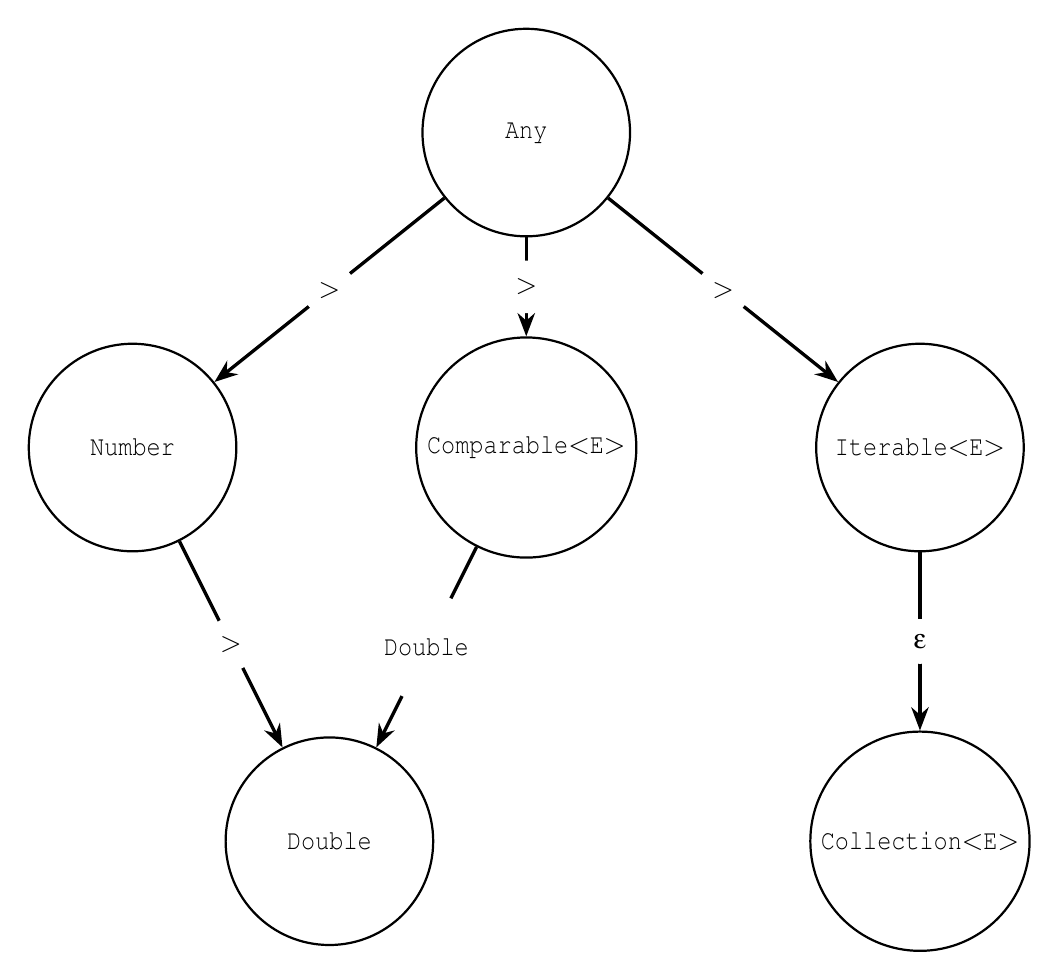
\begin{tikzpicture}
	\begin{scope}[every node/.style={circle,thick,draw} ]
		\node[minimum size=75pt] (D) at (5,4) {\texttt{Any}};
    		\node[minimum size=75pt] (A) at (0,0) {\texttt{Number}};
    		\node[minimum size=75pt] (B) at (5,0) {\texttt{Comparable$<$E$>$}};
    		\node[minimum size=75pt] (C) at (2.5,-5) {\texttt{Double}};
    		\node[minimum size=75pt] (E) at (10,0) {\texttt{Iterable$<$E$>$}};
    		\node[minimum size=75pt] (F) at (10,-5) {\texttt{Collection$<$E$>$}};
	\end{scope}
	\begin{scope}[>={Stealth[black]},
              every node/.style={fill=white,circle},
              every edge/.style={draw=black,very thick}]
    		\path [->] (B) edge node {$\texttt{Double}$} (C);
    		\path [->] (A) edge node {$>$} (C);
    		\path [->] (D) edge node {$>$} (A);
	    	\path [->] (D) edge node {$>$} (B);
    		\path [->] (D) edge node {$>$} (E);
    		\path [->] (E) edge node {$\epsilon$} (F);
%    \path [->] (B) edge[bend right=60] node {$1$} (E); 
	\end{scope}
	\end{tikzpicture}
    \caption{A sample of the type hierarchy representation using standard Kotlin types.}
    \label{fig:type-hierarchy}
\end{figure}


\Cref{fig:type-hierarchy} depicts the \Gls{DAG} representation
a small subset of built-in and standard Kotlin types.
Within this hierarchy, the \texttt{Number}, \texttt{Comparable$<$E$>$}, 
and \texttt{Iterable$<$E$>$} types all directly inherit from the \texttt{Any} node, 
the root of the type hierarchy.
The \texttt{Number} and \texttt{Comparable$<$E$>$} have a common immediate descendant in the 
\texttt{Double} type, though their transitions differ.
The transition between \texttt{Comparable$<$E$>$} and \texttt{Double} itself
contains the annotation \texttt{Double}, an exact type referring to a node in the graph
that is required to complete the inheritance.
The $\epsilon$ label on the edge between \texttt{Iterable$<$E$>$} and \texttt{Collection$<$E$>$}
denotes that \texttt{E} is a symbolic type, and that a link between the two parameterized types
must be consistent.
The meaning of consistency is intricate,
as parameterized types in Kotlin may contain bounds
that further limit the domain of valid parameter types.
To integrate this constraint, bound information is additionally
stored in edge labels.

This representation of types offers several key advantages within the scope of the fuzzer.
First, a graph representation is flexible in that new types can easily be added, removed, or changed
during fuzzing.
This flexibility also enables automating the construction of a type hierarchy
from pre-written Kotlin files, which in turn allows for near-endless customization of the fuzzing space.
Second, a \Gls{DAG} topology enables the encoding of strict semantic constraints into
graph-centric problems.
This applies to simple inheritance semantics
(i.e., subclasses may be used wherever a superclass is expected),
but can also generalize to Kotlin-specific traits,
such as requiring children of the \texttt{Iterable$<$E$>$}
node whenever a \texttt{for} loop occurs.
Finally, the \Gls{DAG} greatly prunes the search space of semantically valid solutions, as simple graph walking
algorithms suffice to solve problems related to sound parameterized type inference, a common problem
when fuzzing the Kotlin standard library.

\subsection{\label{subsec:callables}Callable Representation}
In addition to a type hierarchy, the fuzzer uses knowledge to which \textit{callables}
it can act upon.
We use the term callable in a similar fashion to \citet{stepanov2021type}, with this term encompassing
the set of functions, methods, constructors, variables, constants, and predefined primitive values
available to the fuzzer.
We model each callable as a 5-tuple $\langle N, O, P, I, R \rangle$ that builds on top of the
type hierarchy.
Let $N$ the name of the callable, $O$ the type of the callable's \textit{owner} class,
$P$ a list of (symbolic) parameterized types specific to the callable,
$I$ a list of input types that the callable requires,
and $R$ the return (or output type) of the callable.
This representation draws inspiration from lambda calculus and aims to provide a uniform representation
for all callables that Kotlin can represent.

\lstset{
  basicstyle=\footnotesize, frame=tb,
  xleftmargin=.2\textwidth, xrightmargin=.2\textwidth,
  numbers=left, stepnumber=1,
}

\begin{figure}
\begin{lstlisting}[language=Kotlin]
class Foo <E>(bar: String, baz: E) {
    val fooProp1: String = bar
    var fooProp2: E = baz
    fun <P> fooFunc(parameter: P) : E {
        return fooProp2
    }
}
\end{lstlisting}
\caption{Simple Kotlin snippet.}
\label{fig:callables}
\end{figure}

To help build intuition on the applicability of this representation,
consider the snippet depicted in \Cref{fig:callables}.
Though simple, the \texttt{Foo} class contains several representationally
challenging constructs that help illustrate the capability of the callable construct.
First, the \texttt{Foo$<$E$>$} type itself belongs to the type hierarchy
of the underlying context. 
The \texttt{fooProp1} class property becomes the
$\langle \texttt{fooProp1},$ \texttt{Foo$<$\texttt{E}$>$} $, \emptyset, \emptyset, \texttt{String} \rangle$
quintuple, which is akin to a lambda-calculus function that takes no input and returns a \texttt{String} value.
The \texttt{fooProp2} property is analogous, with the exception of the return type,
which is now a symbolic type \texttt{E}, which is linked to the owner class' parameter type.
During runtime, the fuzzer leverages this link to first determine other contextual constraints
on \texttt{E}, and then sample an appropriate concrete type to fulfill the link.

Finally, the \texttt{fooFunc} method becomes the 
$\langle \texttt{fooFunc},$ \texttt{Foo$<$\texttt{E}$>$} $,
\{ \texttt{P} \}, \{ \texttt{E} \}, \texttt{String} \rangle$
5-tuple, which links both parameter's input type to the method's
own parameterized type \texttt{P} and the return type to the 
class' parameterized type \texttt{E}.
A similar translation occurs for the primary constructor of \texttt{Foo},
which becomes the 
$\langle \texttt{Foo}, \bot, \{ \texttt{E} \}, 
\{ \texttt{String}, \texttt{E} \},$ \texttt{Foo$<$\texttt{E}$>$} $\rangle$
quintuple that takes two inputs and returns an object of type \texttt{Foo$<$E$>$}.
In the latter case, the constructor's owner class is left out,
as a constructor call does not require access to an object.
As in previous cases, the link exist between the \texttt{E} type of 
the callable representation, and the (possibly constrained)
\texttt{E} type in the definition of \texttt{Foo}.

\subsection{\label{subsec:context-extraction}Context Extraction}

To achieve the desired utility, the context representation
must be capable of two fulfilling two core tasks.
First, it should contain sufficient information to enable a fuzzer to generate valid Kotlin
code through successive queries.
Second, it should be flexible enough to support the \textit{extraction} of relevant types
and callables from pre-existing pieces code, without requiring the user to manually
intervene in the process.
The latter requirement drastically increases the applicability of such a tool in
the real world, where practitioners might want to investigate particular language features,
specific implementations of standard interfaces, or proprietary 
code bases. To accomplish this, we developed a three-phase context extraction
process that parses a collection of input Kotlin files and produced a
sound representation using the type hierarchy and callable abstractions.
\Cref{fig:context-extraction} depicts this method.

\def\layersep{0.5}
\def\nodesep{0.5}

\begin{figure*}[!hbtp]
\vspace{2cm}
\centering
\begin{minipage}[t]{-4\linewidth}
\begin{tikzpicture}[transform canvas={scale=1.0},node/.style={circle, draw, thick}]

\foreach \Z in {0,0.5,1,1.5}
 {\draw[fill=gray,draw=black] (-6,0,\Z) rectangle (-5.25,1,\Z);}

\node[] at (-5.5,1.5)   (a) {Input Files};

 \draw [-stealth] (-5, 0.5) -- node[pos=0.5,above]{Parsing} (-3.5, 0.5);
 
 \pgfmathsetmacro{\cubex}{1}
\pgfmathsetmacro{\cubey}{1}
\pgfmathsetmacro{\cubez}{1}

\node[node] (pt1) at (-3,1,0) {};
\node[node] (pt2) at (-3,0.5,0) {};
\node[node] (pt3) at (-3,0,0) {};

\path[-stealth, thick] (pt1) edge (pt2);
\path[-stealth, thick] (pt2) edge (pt3);

\node[node] (pt5) at (-2.5,1,0) {};
\node[node] (pt6) at (-2.5,0.5,0) {};
\node[node] (pt7) at (-2.5,0,0) {};

\path[-stealth, thick] (pt5) edge (pt6);
\path[-stealth, thick] (pt6) edge (pt7);

\node[] at (-2.75,1.875)   (a) {Parse trees};

\draw [-stealth] (-2, 0.5) -- node[pos=0.5,above]{Traversal} (-0.5, 0.5);

\draw[black,fill=gray] (0.75,1,0) -- ++(-\cubex,0,0) -- ++(0,-\cubey,0) -- ++(\cubex,0,0) -- cycle;
\draw[black,fill=gray] (0.75,1,0) -- ++(0,0,-\cubez) -- ++(0,-\cubey,0) -- ++(0,0,\cubez) --  cycle;
\draw[black,fill=gray] (0.75,1,0) -- ++(-\cubex,0,0) -- ++(0,0,-\cubez) -- ++(\cubex,0,0) -- cycle;

\node[] at (0.5,1.875)   (a) {IR};

\draw [-stealth] (1.25, 0.5) -- node[pos=0.5,above]{Sorting} (3.25, 0.5);

  \foreach \y in {1,...,3}{
      \node[node] (i\y) at (3.75,\nodesep*\y-0.5) {};
      \node[node, right=\layersep of i\y] (h1\y) {};
      \node[node, right=\layersep of h1\y] (h2\y) {};
    }

  \foreach \source in {1,...,3}
  \foreach \dest in {1,...,3}{
      \path[-stealth, thick] (i\source) edge (h1\dest);
      \path[-stealth, thick] (h1\source) edge (h2\dest);
    }

\draw[] (3.35, -0.5) rectangle (5.85, 1.5);

\node[] at (4.6,1.875)   (a) {Type DAG};


 %%%%%%%%%%%%%%%%%%%%%%%%%%%% Bottom half
\draw [-stealth] (0.5, -0.25) -- (0.5, -2) -- (1.3, -2);
\draw [-stealth] (4.6, -0.55) -- (4.6, -2) -- (3.15, -2);

\draw[black,fill=gray] (2.55,-1.5,0) -- ++(-\cubex,0,0) -- ++(0,-\cubey,0) -- ++(\cubex,0,0) -- cycle;
\draw[black,fill=gray] (2.55,-1.5,0) -- ++(0,0,-\cubez) -- ++(0,-\cubey,0) -- ++(0,0,\cubez) --  cycle;
\draw[black,fill=gray] (2.55,-1.5,0) -- ++(-\cubex,0,0) -- ++(0,0,-\cubez) -- ++(\cubex,0,0) -- cycle;

\node[] at (2.3,-3)   (a) {Callables};


\end{tikzpicture}
\end{minipage}
\vspace{3.5cm}
\caption{Simplified visualization the context extraction process.}
\label{fig:context-extraction}
\end{figure*}

The extraction process operates on a parsed representation of the input
files, which for the scope of this research consists built-in and standard library 
Kotlin files.
The first phase traverses the parse trees of the Kotlin files and maps
relevant information into an intermediate representation.
The retained information includes the necessary details to identify language constructs,
available types, and relations between parameterized types.
The second step then creates the links between 
parameterized types in class declarations and their properties, while simultaneously
traversing the intermediate representation and inserting metadata with regarding
visibility and inheritance modifiers.

The third step of the procedure involves building the type hierarchy \Gls{DAG}.
At this point, extracted class definitions contain links that allow for the
differentiation between symbolic and concrete types, which makes resolving
inheritance relations possible.
Because of this, a simple topological sorting algorithm suffices to construct the \Gls{DAG}.
An initial \texttt{Any} node serves as the root of the graph
and represents the parent for all classifiers
that do not explicitly inherit from other constructs.

\newacronym{OO}{OO}{Object-Oriented}

This design choice simplifies the application of further graph traversal algorithms.
The topological sorting then proceeds by filtering available parsed classifiers on three conditions: (i) that the direct parents of the classifier have been added to the hierarchy, (ii) that the concrete parameterized types of the classifier have been added to the hierarchy, and (iii) that the owner
type of the classifier has been added to the hierarchy (if nested types are encountered).
Classifiers that meet these requirements can be added in an arbitrary order.
The algorithm then proceeds until all visible classifier types have been processed.
This stopping condition places the burden of selecting a sound
subset of input files on the user.
However, we provide a subset of Kotlin standard library files as
a sensible default option.

Once a type hierarchy has been established, the final step creates links between the
processed types and the relevant callables.
Each intermediate representation of a callable receives a copy of its owner's type
before being converted into its final representation, which enables conversion to
valid Kotlin code.
The context tracks each callable by its owner's type, with a special empty owner for built-in 
functions.
This method of storage not only models the intuitive structure of \Gls{OO} code 
(with container classes and their properties), but decreases the complexity of
common queries during runtime.

\section{\label{sec:syntax}Syntactic Interface}

Effectively leveraging the syntax of a programming language is of paramount importance
ensuring the correctness of automatically generated code.
In this work, we seek to exploit the usage of the Kotlin \gls{CFG} as both a means of increasing
the flexibility of the fuzzer and a guide that enforces the validity of generated code.
This places our fuzzing approach in the \textit{grammar-aided} category defined by 
\citet{chen2020survey}.

Though highly informative, a \gls{CFG}-based model of linguistic syntax
suffers from several limitations which
curtail the grammar's standalone potential within the fuzzer.
The remainder of this section describes the
implementation of the grammatical representation
within the fuzzer, its integration with the Context,
and the reasons behind the enhancements
we enriched the grammar with.

\subsection{\label{subsec:extending-cfg} Extending the Kotlin CFG}

In attempting to enhance the contextual integration of the Kotlin \gls{CFG},
it is important to consider its practical setbacks.
The Kotlin developer team provides a standard grammar specification \cite{kotlingrammar},
implemented using the \textsc{antlr4} framework.
\textsc{antlr4} \cite{parr2013definitive} is parser generator that
offers a broad range of language-targeted functionality,
including the validation and structured parsing of input
with respect to a given grammar.

The available grammar implementation encapsulates a highly complex 
and finely detailed set of rules.
In its current form, the \gls{CFG} consists of two components - a Lexer grammar
and a Parser grammar.
The former pertains to the lower-level components of the Kotlin language, 
including keywords, symbols, and numerical representations, split between 315 
symbols and 378 productions.
The latter models the higher-level constructs of the language, ranging from
simple statements to class definitions, and totals 170 variables and 353 rules.

Altogether, the two compartments create a substantial collection of non-trivial
of syntactic constraints, the complexity of which increases with each nested
relation.
In practice, this complexity causes straight-forward specification fuzzing algorithms
(such as, for instance, traversing the grammar)
to generate semantically invalid Kotlin code with overwhelming likelihood.
This in turn imposes massive challenges on any fuzzer attempting to utilize these
rules in any substantial sense.
An implementation of grammar-aided techniques requires a
solution that reduces the likelihood of generating invalid code by sampling grammar productions.

To fulfill this requirement, we propose an approach that \textit{extends} the core
Kotlin \gls{CFG} with an enhanced representation that circumvents several key shortcomings.
The transformation from the barebones \gls{CFG} to its extended version takes place
at the node (symbol) level in  the graph representation, as to improve comprehension.
To obtain this transformation, we use a traversal algorithm which takes as input the
\textsc{antlr4} core-grammar node and outputs its enhanced version.
This algorithm performs a single key operation for each symbol:
it endows each node in the core \gls{CFG} with a grammar-abiding \texttt{sample} property,
which aims at reducing the complexity of generating valid samples.
The atomic node transformation can either leave a node unchanged or \textit{truncate} its
productions.
Simple nodes such as ones solely containing unicode characters are preserved, while
nodes which introduces substantial contextual semantics are subject to change.
This reduces the problem of obtaining valid samples from the grammar to implementing
appropriate methods of leveraging the \texttt{sample} property of each affected node.

\begin{figure}
    \centering
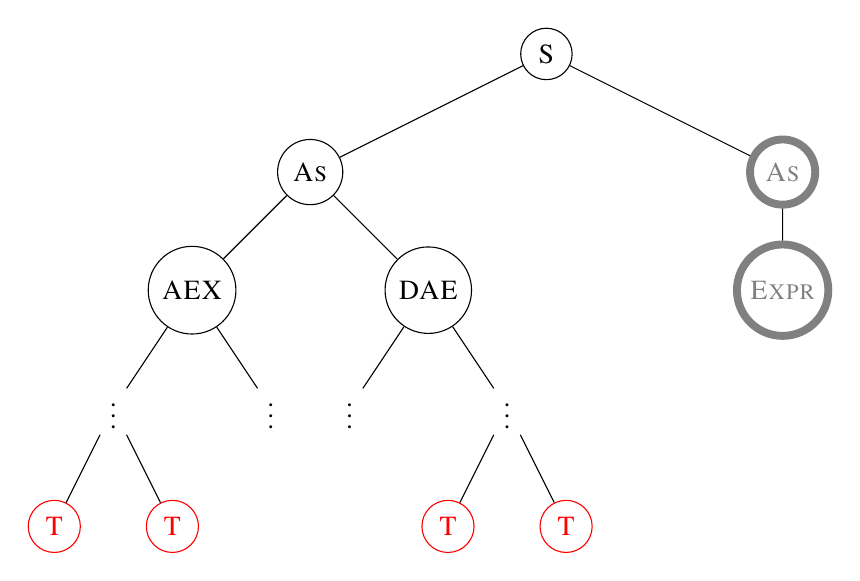
\begin{tikzpicture}[level/.style={sibling distance=60mm/#1}]
\node [circle,draw] (z){\textsc{S}}
  child {node [circle,draw] (a) {\textsc{As}}
    child {node [circle,draw] (b) {\textsc{AEX}}
      child {node {$\vdots$}
        child {node [circle,draw,color=red] (d) {\textsc{T}}}
        child {node [circle,draw,color=red] (e) {\textsc{T}}}
      } 
      child {node {$\vdots$}
      }
    }
    child {node [circle,draw] (g) {\textsc{DAE}}
      child {node {$\vdots$}}
      child {node {$\vdots$}
      child {node [circle,draw,color=red] (d) {\textsc{T}}}
        child {node [circle,draw,color=red] (e) {\textsc{T}}}
        }
    }
  }
%  child {node [circle,draw] (j) {\textsc{As}}
    child {node [circle,draw,color=gray,line width=1mm] (k) {\textsc{As}}
        child {node [circle,draw,color=gray,line width=1mm] (l) {\textsc{Expr}}}
%    }
};
\end{tikzpicture}
 \caption{Sample \gls{CFG} transformation.}
    \label{fig:extended_cfg}
\end{figure}

\Cref{fig:extended_cfg} depicts an example of a transformation performed
on a section of the Kotlin grammar.
In this scenario, the root node \textsc{s} represents a \textit{statement} in the Kotlin
language and directly maps to a symbol in the core \gls{CFG}.
The symbol \textsc{s} could follow a production to sample an \textit{assignment}
node \textsc{as} as depicted in the left half of the figure.
This rule introduces additional semantic constraints, which the grammar omits.
The \textsc{as} node may be extended into either
an assignable expression (\textsc{aex}) or 
a directly assignable expression (\textsc{dae}), the details of which are
not important for the sake of this example.
Either production can in turn unravel into a chain of derivations that eventually
sample terminal nodes \textsc{t}.
Following this series of derivations, the semantic constraints that the production
$\textsc{s} \to \textsc{as}$ entails (such as type consistency in the assignment)
do not propagate to further links in the chain,
and thus the likelihood of generating
valid code by trivially sampling terminal nodes in the derivation
is vanishingly small.

The transformed grammar shown on the right branch of the \textsc{s} symbol circumvents
this problem by truncating the grammar at the node that introduces such constraints.
In this case, the algorithm transforms \textsc{as} node into its extended version,
which encodes relevant constraints within its \texttt{sample} property.
Transformed nodes may additionally transfer such constraints between them when sampled:
for instance, the assignment node may propagate its type-consistent constraint to a generic
\textsc{expr} node that generates consistent and valid Kotlin expressions.

This extended \gls{CFG} technique provides several advantages.
First, it forms a framework that solves the problem of semantically constrained grammar sampling.
By implementing the appropriate \texttt{sample} properties,
one can effectively evade the problems that the context-invariant grammar raises.
Second, it is an effective trade-off between implementation difficulty and core grammar usage. 
This technique preserves the key properties and relations in the Kotlin grammar, while
not necessitating that every production is individually catered to. 
For instance, transformed nodes may simply inherit (part of) their structure from the
\textsc{antlr4} definition.

Finally, the extended \gls{CFG} framework serves as a versatile foundation for fuzzing
algorithms, by allowing higher-level routines to target specific symbols in the grammar.
This property may prove valuable as practitioners could use heuristics to stress 
certain language features, compiler modules, or code bases in a more reliable
manner than depending on sheer randomness.

This approach stands out from the current body of literature through 
the balance it strikes between the level of user "intervention" in re-writing grammar
rules and the utilization of pre-written grammar specifications.
In isolation, neither side of this this trade-off is novel.
\textsc{Csmith} \cite{yang2011finding} has demonstrated the effectiveness
of manually constructing a sampling structure without
direct usage of a grammar over a decade ago, while approaches like
\textsc{ISLa} \cite{steinhofel2022input} show that
constrain-annotated grammars can effectively encode
common and meaningful semantic constraints.
However, our integration of contextual sampling within an extended
grammar representation enables algorithms built on top of it
to individually tune the semantic constraints of each individual
symbol, while always having to option to "fall back" on the 
pure grammar representation in cases where appropriate.
\subsection{\label{subsec:context-efcg} Connecting Context and Grammar}


To fully leverage their \texttt{sample} property, nodes in the 
extended grammar representation require an extensive connection to their local context.
To facilitate this arrangement, the we connect the initial (or \textit{root})
context to the node from which sampling starts.
As sampling algorithms recursively visit nodes in the extended grammar,
additional information embedded in each node helps the traversal decide
whether the current context should be transmitted as-is, cloned, or mutated.

Simple nodes like expressions utilize an unchanged context, while more complex
constructs, like variable declarations may insert additional identifiers.
Encompassing constructs like class and function definitions are scope sensitive,
which requires careful handling local and nested operations.
To address this, each such node creates a local copy of the context, to
which it might add isolated information, before persisting globally accessible data
(i.e., function names, or new types) to the root context.
In essence, this integration allows for autonomous context-sensitive random sampling from the 
extended grammar: the extended nodes each query the context
in such a way that consistent constructs emerge.
The context, in turn, provides an interface that provides several guarantees with respect 
to future future parameterized queries.

\section{\label{sec:repr} Code Representation}

To facilitate the implementation of measurable 
optimization criteria, we propose a versatile \gls{GA}-based framework
that supports common evolutionary search operators.
Such a framework requires a central representation of Kotlin code that is
granular enough to leverage the rich semantic information accessible through
the context, and simple enough to support large numbers of operator
calls during search.
To achieve this, we designed a hierarchical chromosomal representation
that distinguishes between three levels of separation.

The hierarchy roots itself in a tri-level
complexity abstraction that discerns between pieces of code
based on scope and isolated validity.
\Cref{fig:code-hierarchy} illustrates this hierarchy.
\textit{Fragments} lie at the base of the pyramid and compose low-level 
language constructs, such as expressions and statements.
These pieces of code are of low independent value as they do not
capture any logic structure and rely heavily on surrounding semantic context.
A step above are the code \textit{snippets}: individually encapsulated
pieces of code comprised of fragments.
Snippets emerge when changes in scope are significant enough to
merit a logical separation.
Such scenarios generally occur along the lines of \gls{OO} design,
and include functions, methods, and classes.


\begin{figure}[htp]
\centering
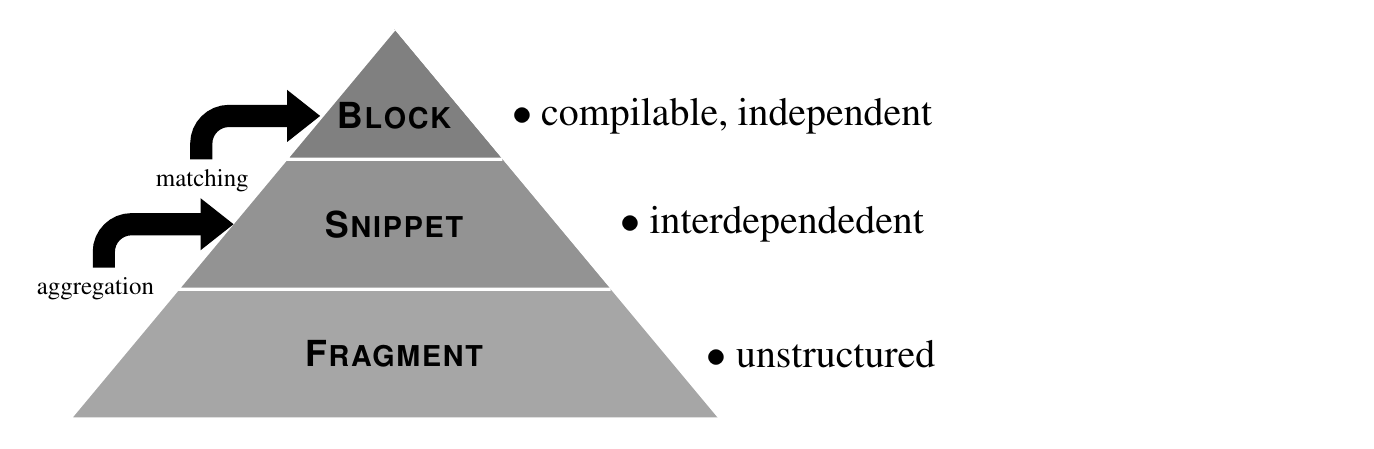
\begin{tikzpicture}[scale=0.55]
        \filldraw[very thick,white,fill=gray!70] (0,0) -- (-7.5,-9) -- (7.5,-9);
        \filldraw[very thick,white,fill=gray!85] (0,0) -- (-5,-6) -- (5,-6);
        \filldraw[very thick,white,fill=gray] (0,0) -- (-2.5,-3) -- (2.5,-3);
        \node at (0,-2) {\bfseries\sffamily\scshape\Large Block};
        \node at (0,-4.5) {\bfseries\sffamily\scshape\Large Snippet};
        \node at (0,-7.5) {\bfseries\sffamily\scshape\Large Fragment};
        \node[text width=8cm] at (10,-2) {\Large $\bullet$ compilable, independent};
        \node[text width=8cm] at (12.5,-4.5) {\Large $\bullet$ interdependedent};
        \node[text width=8cm] at (14.5,-7.5) {\Large $\bullet$ unstructured};
    \begin{scope}[xshift=-3.7cm,yshift=-3cm]
        \draw[-{Triangle[width=18pt,length=12pt]}, line width=8pt, rounded corners=10pt, black] (-0.75,0) -- (-0.75,1) -- (2,1);
        \node[text width=5cm] at (2.75,-.5) {\small matching};
    \end{scope}
    \begin{scope}[xshift=-5.7cm,yshift=-5.5cm]
        \draw[-{Triangle[width=18pt,length=12pt]}, line width=8pt, rounded corners=10pt, black] (-1,0) -- (-1,1) -- (2,1);
        \node[text width=5cm] at (2,-.5) {\small aggregation};
    \end{scope}
\end{tikzpicture}

 \caption{Representational hierarchy of code complexity abstractions.}
 \label{fig:code-hierarchy}
\end{figure}

Snippets serve as an intermediate layer that captures sufficient information to be individually actionable (i.e., a function that can be called), but not enough to be
context-independent.
The interdependency of snippets materializes as a consequence of
the sequential nature of node sampling: as nodes recursively unfold
their \texttt{sample} property, prior changes to the context
trigger subsequent effects (i.e., previously generated 
functions may appear in later expressions).
To overcome this obstacle several snippets can assemble into \textit{blocks},
the highest construct of the pyramid.
This snippet \textit{aggregation} procedure works on the basis of a dependency matching
algorithm that recursively traverses snippets within a Kotlin file and retrieves
external snippets that their fragments depend on.
The pyramidal abstraction construct shares conceptual similarities with both
the works of \citet{holler2012fuzzing} and \citet{han2019codealchemist}.
However, there are fundamental differences between our method and past work.
Unlike \citet{holler2012fuzzing}, more sophisticated, language-targeted
generation procedures serve as the basis of novel code blocks, which do not
rely on input seed programs.
The aggregation of snippets into blocks also differs from the semantics-aware
assembly proposed by \citet{han2019codealchemist}, which infers language constraints
from a corpus of over 200,000 files.
Our approach requires no such input, making the generation process entirely self-sustaining. 

\Cref{fig:blocks} exemplifies the differences between the three levels
of the hierarchy.
The statements in lines 2 and 6, as well as the expression
in line 10 are all instances of \textit{fragments}: pieces
of code that too small to track in the model.
The functions \texttt{x}, \texttt{y}, and \texttt{z} are all \textit{snippets}:
independently separable pieces of code that are not necessarily self-sufficient.
Finally, there are three \textit{blocks} in this example: $\langle \texttt{x} \rangle$,
$\langle \texttt{x}, \texttt{y} \rangle$,
and $\langle \texttt{x}, \texttt{y}, \texttt{z} \rangle$.
All three of these blocks share the property that they are context-independent:
the dependencies for all snippets in the block are also part of the block.
Preserving this property during search is critical not only because it is the most
effective way of employing the context's semantic guarantees,
but also because it ensures that compiler resources do not go to waste
in analyzing incomplete files.
The \textit{block} abstraction is the cornerstone of the 
\gls{GA} framework, shaping all higher-level operators and constructs.

\begin{figure}
\begin{lstlisting}[language=Kotlin]
fun x() : Double {
	return 0.0
}

fun y() : Double {
	return x() + 1.0
}

fun z() {
	return y()
}
\end{lstlisting}
\caption{Illustration of fragments, snippets, and blocks.}
\label{fig:blocks}
\end{figure}

\paragraph{Individuals.} The population of the \gls{GA} consists
of individual \textit{blocks} encoded in a chromosomal representation as follows.
A chromosome consists of a list $\mathcal{L}$ of triples
$\mathcal{S} := \langle \mathcal{R}, \mathcal{D}, \mathcal{T} \rangle$ representing snippets,
with $\mathcal{R}$ a representation of the signature of the snippet,
$\mathcal{D}$ a list of signatures of snippets that $\mathcal{S}$ depends on,
and $\mathcal{T}$ the text that the snippet contains.
Considering again the code in \Cref{fig:blocks},
the chromosome encoding the block $\langle \texttt{x}, \texttt{y} \rangle$
is $\mathcal{L}_{\langle \texttt{x}, \texttt{y} \rangle} =
[ \langle
\texttt{x} : \lambda \to \texttt{Double}, \emptyset, \mathcal{T}_{\texttt{x}}\rangle,
\langle \texttt{y} : \lambda \to \texttt{Double},
\{ \texttt{x} : \lambda \to \texttt{Double} \}, \mathcal{T}_{\texttt{y}} \rangle ]$
The first entry in the list models the \texttt{x} function, with a
$\lambda$-calculus inspired signature, an empty dependency set, and
the first lines 3 of the code.
The second entry is analogous, except for the dependency set 
that contains the signature of \texttt{x}, signaling that
lines of code 5-7 require the presence of \texttt{x} for completeness.

\paragraph{Context-Aware Partitioning.} A downside of the
established chromosome model has to do with the ordering of
snippets inside $\mathcal{L}$.
Though representationally irrelevant, the order of snippets within
the list becomes relevant when the chromosome instantiates
a concrete piece of code.
Snippets in Kotlin can be order-sensitive, meaning that to
instantiate valid code, the list of snippets within the chromosome
should be arranged such that a topological dependency structure
emerges.
Using again the example in \Cref{fig:blocks}, this means
that within the chromosome representing the entire piece of code,
the snippet \texttt{x} must always be precede \texttt{y} and \texttt{z}.
Similarly, \texttt{y}, must always appear before \texttt{z}.

There are several ways to achieve this ordering.
Since the generative process is iterative, the first instantiation
of a block always obeys this constraint.
However, preserving this property during the application of
variation operators proves more challenging.
To effectively mutate and recombine individuals,
blocks require the capability of
identifying entire dependency structures centered around particular snippets.
In other words, given a snippet \texttt{s} present in a block
\texttt{b}, \texttt{b} should be able to  identify a \textit{partition}
of itself that includes (i) \texttt{s}, (ii) all snippets
that depend on \texttt{s}, and (iii) all downstream dependencies of (i) and (ii).
We refer to a partition that such a structure as a \textit{self-sufficient} partition
of a block.

To build such a partition starting from an arbitrary snippet
requires careful analysis of the dependency structure within a block.
To implement this, we propose a technique that models the
structure of a block as a \textit{dependency graph}, a common
data structure used in static analysis of programs.
Each node \texttt{n} represents a snippet within the block,
and each directed edge $\texttt{n}_1 \to \texttt{n}_2$
denotes that snippet $\texttt{n}_1$ depends on $\texttt{n}_1$.
To construct a self-sufficient partition starting from a node $\texttt{n}$,
we employ two procedures that traverse the dependency graph
to gather information regarding its topology.
An \textit{upstream} traversal starting at \texttt{n} walks
along every possible path \textit{ending} in \texttt{n}, in
effect gathering all blocks that either directly or indirectly depend on \texttt{n}.
Reflexively, a \textit{downstream} traversal beginning at \texttt{n}
walks on every path originating in \texttt{n} and gathers all of \texttt{n}'s
dependencies.

\Cref{fig:traversals} depicts several sample traversals of a
snippet dependency structure similar to that introduced in \Cref{fig:blocks}.
Subfigure (a) gives the standalone topology of the block, and selects
snippet \texttt{y} as the root of the traversal.
An upstream traversal rooted in \texttt{y} would select \texttt{b} and \texttt{z},
which directly depend on \texttt{y}, as depicted in panel (b).
A downstream traversal rooted in \texttt{y} would additionally yield
snippet \texttt{x}, which is \texttt{y}'s only direct dependency, as shown in 
subfigure (c).
Finally, it is important to note that the repeated application of up- and downstream
traversal on increasingly larger sets of nodes (i.e., each traversal considers \textit{all}
nodes returned by the previous) yields the largest connected subgraph containing the
original starting node.
Subfigure (d) illustrates three such traversals:
starting at \texttt{a}, \texttt{b} is selected during an upstream traversal.
Next, \texttt{y} and \texttt{x} from the downstream traversal rooted at \texttt{b}.
Lastly, an upstream traversal rooted at either \texttt{x} or \texttt{y} yields \texttt{z}.
The additional benefit of such traversals is that they preserve
the ordering of nodes in graph, which graph walking algorithms may fail to do.

\begin{figure}[t!]
\centering
\subfigure[Initial choice of snippet.]{
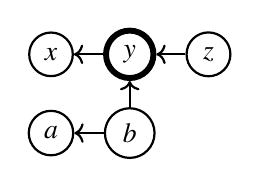
\begin{tikzpicture}[node distance={10mm}, thick, main/.style = {draw, circle}] 
\node[main] (1) {$x$}; 
\node[main, line width=0.75mm] (2) [right of=1] {$y$}; 
\node[main] (3) [right of=2] {$z$}; 
\node[main] (4) [below of=1] {$a$}; 
\node[main] (5) [right of=4] {$b$};  
\draw[->] (2) -- (1);
\draw[->] (3) -- (2);
\draw[->] (5) -- (2);
\draw[->] (5) -- (4);
\end{tikzpicture}}
\hfill
\subfigure[Upstream traversal from \texttt{y}.]{
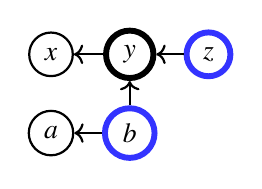
\begin{tikzpicture}[node distance={10mm}, thick, main/.style = {draw, circle}] 
\node[main] (1) {$x$}; 
\node[main,line width=0.75mm] (2) [right of=1] {$y$}; 
\node[main,draw=blue!80,line width=0.75mm] (3) [right of=2] {$z$}; 
\node[main] (4) [below of=1] {$a$}; 
\node[main,draw=blue!80,line width=0.75mm] (5) [right of=4] {$b$};  
\draw[->] (2) -- (1);
\draw[->] (3) -- (2);
\draw[->] (5) -- (2);
\draw[->] (5) -- (4);
\end{tikzpicture}
}
\hfill
\subfigure[Downstream traversal from \texttt{y}.]{
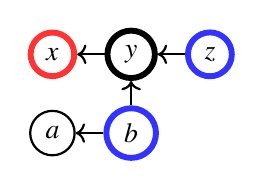
\begin{tikzpicture}[node distance={10mm}, thick, main/.style = {draw, circle}] 
\node[main,draw=red!80,line width=0.75mm] (1) {$x$}; 
\node[main,line width=0.75mm] (2) [right of=1] {$y$}; 
\node[main,draw=blue!80,line width=0.75mm] (3) [right of=2] {$z$}; 
\node[main] (4) [below of=1] {$a$}; 
\node[main,draw=blue!80,line width=0.75mm] (5) [right of=4] {$b$};  
\draw[->] (2) -- (1);
\draw[->] (3) -- (2);
\draw[->] (5) -- (2);
\draw[->] (5) -- (4);
\end{tikzpicture}
}
\hfill
\subfigure[Successive up-, down-, and upstream traversals starting at \texttt{a}.]{
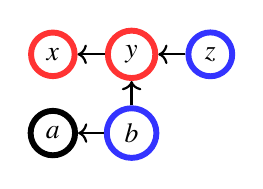
\begin{tikzpicture}[node distance={10mm}, thick, main/.style = {draw, circle}] 
\node[main,line width=0.75mm,draw=red!80] (1) {$x$}; 
\node[main,line width=0.75mm,draw=red!80] (2) [right of=1] {$y$}; 
\node[main,line width=0.75mm,draw=blue!80] (3) [right of=2] {$z$}; 
\node[main,line width=0.75mm] (4) [below of=1] {$a$}; 
\node[main,line width=0.75mm,draw=blue!80] (5) [right of=4] {$b$};  
\draw[->] (2) -- (1);
\draw[->] (3) -- (2);
\draw[->] (5) -- (2);
\draw[->] (5) -- (4);
\end{tikzpicture}
}
\caption{Sample upstream and downstream traversals of snippet dependencies. Nodes with thick borders are affected by the traversal, while thinly bordered ones are not. Black depicts that the node is the starting point of the traversal, while blue and red denote nodes selected during up- and downstream traversals, respectively.}
\label{fig:traversals}
\end{figure}

\paragraph{Mutation.} To fully take advantage of the properties of blocks,
mutation operators must ensure the preservation self-sufficiency.
Since perturbing the dependency hierarchy within blocks
would render any validity guarantees pointless, we designed
mutation procedures to operate on partitions of code blocks selected by 
means of the previously established traversals.
This includes three mutation varieties:

\begin{itemize}
	\item \textbf{Removal} of a selected partition. This operator first chooses a random 
	snippet within the block and performs an upstream traversal from that snippet.
	The operator then removes all collected snippets from the chromosome.
	\item \textbf{Context-Free Addition} performs a sample operation
	on the node that the given block originates from, and appends the result to the end
	of the chromosome.
	\item \textbf{Context-Aware Addition} first brings the context in a state
	that is compatible with the block subject to mutation, and then performs a sample
	operation. The result extends the chromosome as in the context-free case.
\end{itemize}

\paragraph{Recombination.} We propose a simple recombination operator
that takes in a pair of chromosomes $\mathcal{L}_{p_1}$ and $\mathcal{L}_{p_2}$
and creates two offspring  $\mathcal{L}_{o_1}$ and $\mathcal{L}_{o_2}$.
The offspring start out as identical copies of each parent, before
crossover swaps two collections of snippets between them.
The collection of snippets emerges using repeated up- and downstream
traversals initially rooted a randomly chosen snippet in the block.
The resulting selections preserve both the self-sufficiency and
ordering constraints of both the extracted and remaining partitions.
As a result, the selected partitions of each block are swapped and appended
to the opposite chromosome.

\paragraph{Selection.} We provide standard selection operators for both
single- (tournament and proportionate selection) and
multi-/many-objective (domination rank and domination count selection) fitness functions.
\\\\
To exploit the power of this framework to its full extent,
we allow for a large degree of external configuration.
The remainder of this section covers three meta-heuristic
strategies implemented on top of this general framework and analyzes
their merits and potential.


\section{\label{sec:heuristics}Generative Heuristics}

The semantic, syntactic, and representational interfaces
described in Sections \ref{sec:context}, \ref{sec:syntax}, and \ref{sec:repr}
lay the foundation for more complex overarching heuristics
to guide a generative process underlying fuzzing.
This section explores four meta-heuristic guiding oracles shaped into
several concrete algorithm variations and their application
in the context of compiler fuzzing.
Subsections \ref{subsec:random-sampling}, \ref{subsec:diversity-ga}, and
\ref{subsec:proximity-ga} elaborate three compiler-free heuristics, while \ref{subsec:compiler-ga} describes the integration of the compiler within the established heuristics.


\subsection{\label{subsec:random-sampling} Random Sampling}

\newacronym{RS}{RS} {Random Sampling}

Perhaps the simplest method to leverage the context and grammar constructs
is to repeatedly sample a given node in the extended grammar by traversing a
context-informed random node path.
We refer to this generative procedure as \Gls{RS}.
Though trivial in its scope, this approach has proven deceptively powerful
and is the dominant search strategy employed in some shape by all state-of-the-art
fuzzers discussed in \Cref{sec:compiler_testing}.
Despite its simplicity, \gls{RS} establishes a powerful interface, which
all algorithms involved in this study follow.
\Cref{alg:rs} describes the \gls{RS} procedure.

\begin{algorithm}

	\SetKwData{Left}{left}
	\SetKwData{This}{this}
	\SetKwData{Up}{up}
	\SetKwFunction{init}{InitializeAndEvaluatePopulation}
	\SetKwFunction{terminate}{ShouldTermiante}
	\SetKwFunction{offspring}{CreateAndEvaluateOffspring}
	\SetKwFunction{select}{SelectIndividuals}
	\SetKwFunction{time}{TimeElapsed}
	\SetKwFunction{clone}{Clone}
	\SetKwFunction{sample}{Sample}
	\SetKwInOut{Input}{Input}
	\SetKwInOut{Output}{Output}
	\Input{Node to sample $\mathcal{N}$, Context $\mathcal{C}$, Time Budget $s$}
	\Output{Collection of generated Kotlin files}
	\BlankLine
	\DontPrintSemicolon
	%\emph{special treatment of the first line}\;
	$A \gets \emptyset$\;
	\While{$\neg$ \time{$s$}}{
		$c \gets \clone {$\mathcal{C}$}$\;
		$b \gets \sample {$\mathcal{N}$, c}$\;
		$A \gets A \cup \{ b \}$\;
	}
	\Return $A$\;

	\caption{Random Sampling}
	\label{alg:rs}
\end{algorithm}


The sampling procedure takes as input a node $\mathcal{N}$, a context $\mathcal{C}$, 
and a time budget $s$ that determines how long to run for.
The loop simply invokes the target node's \texttt{sample} property repeatedly,
generating code that is syntactically rooted in the target.
Since this procedure mutates the provided context, the main loop creates a fresh
clone of original context $\mathcal{C}$ to prevent cross-referencing between
different files.
An archive $A$ tracks and collects each generated file.
The procedure finishes it exhausts the allotted time budget,
and the output consists of all the generated files.

The proven effectiveness of random sampling as a generative mechanism
in conjunction with a \gls{BB} treatment of the target compiler
has lead researchers to focus on developing auxiliary methods
in support of the core random search driving mechanism.
As a result, many of today's compiler fuzzing tools utilize heuristics to shape
the direction of stochastic sampling procedures rather than directly
optimize solutions for these objectives.
The remainder of this chapter explores auxiliary optimization settings,
that seek to substitute the standard \gls{RS} procedure
with directly measurable objectives.

\subsection{\label{subsec:diversity-ga}Syntactic Diversity-Driven Search}

Generating code that covers a broad range of the Kotlin
input space is a key challenge for thoroughly exercising the many features
of the compiler.
This subsection delves into two ways a \gls{GA} can model, measure,
and optimize for the diversity of its generated files, with the goal
of triggering varied internal compiler behavior.

\subsubsection{\label{subsec:model-div} Modeling Syntactic Diversity} Diversity is intrinsically linked to the
concept of (dis)similarity.
To effectively build such a notion in the domain of semantically
complex Kotlin code, the fuzzer requires a transformation capable
of mapping Kotlin blocks to a space embedded with
a notion of distance.
For this purpose, we opted to measure the number of distinct
language constructs that each block contains.
To this end, the grammar sampling process actively tracks
its stochastic traversal of the \gls{CFG} graph such that
each new occurrence of a node causes a dedicated counter to increment.

Once generation has concluded, the newly established block
internally maintains a vectorized numerical representation of
all its counters.
This simplified representation implicitly describes a 
coordinate space that contains every possible valid piece of Kotlin space
(though, clearly, many semantically dissimilar pieces of code can be mapped to the same points).
Furthermore, this syntactically-minded space largely overlooks
the semantic nuances of the blocks that inhabit it, driving the genetic process
almost entirely through the \gls{CFG}.
This is key for promoting structurally diverse blocks in the population.

\newacronym{SO}{SO} {Single-Objective}

\subsubsection{\label{subsec:soga}Direct Single-Objective Diversity Optimization}

We integrate the
diversity model into the \gls{GA} framework by means of a custom \gls{SO} fitness function.
Let $b_1$ and $b_2$ be two code blocks, generated using the procedure
described in the previous paragraphs.
Let $m : \mathcal{B} \to \mathbb{N}^{k}$ be the mapping that operates
on the input space of all possible blocks $\mathcal{B}$ and outputs
a $k$-dimensional vector of natural numbers representing, for each position,
the number of language structures of a certain type present within the block.
Using this mapping, any common measure of distance
$d : \mathbb{N}^k \times \mathbb{N}^k \to \mathbb{R}$ may be used to determine
the distance between two blocks.
Within this framework, we equate the distance between two blocks to a
simplified notion of similarity.
From these conventions, the notion of population-wide 
similarity follows:

\begin{equation}
dis(b, P) = min_{b^{(i)} \in P - \{ b \}} \{ d(m(b), m(b^{(i)})) \}
\label{eq:sim}
\end{equation}


Intuitively, the similarity of a block $b$ with regard to a population
$P$ is the minimum distance from $b$ to a different block $b^{(i)}$
belonging to the population. 
This notion gives rise to a population-wide diversity fitness function:

\begin{equation}
\min_{b \in \mathcal{B}} f^{(SO)}_{\texttt{DIV}}(b, P) = \frac{1}{1 + dis(b, P)}
\end{equation}

\begin{algorithm}[t]

	\SetKwData{Left}{left}
	\SetKwData{This}{this}
	\SetKwData{Up}{up}
	\SetKwFunction{init}{InitializeAndEvaluatePopulation}
	\SetKwFunction{terminate}{ShouldTermiante}
	\SetKwFunction{offspring}{CreateAndEvaluateOffspring}
	\SetKwFunction{select}{SelectIndividuals}
	\SetKwFunction{time}{TimeElapsed}
	\SetKwFunction{clone}{Clone}
	\SetKwFunction{sample}{Sample}
	\SetKwInOut{Input}{Input}
	\SetKwInOut{Output}{Output}
	\Input{Population size $n$, Node to sample $\mathcal{N}$, Context $\mathcal{C}$, Time Budget $s$}
	\Output{Collection of generated Kotlin files}
	\BlankLine
	\DontPrintSemicolon
	$t \leftarrow 1$\;
	$P_1 \leftarrow $ \init{$n, \mathcal{N}, \mathcal{C}$}\;
	$P^{*} \leftarrow P_1$\;
	\While{$\neg$ \time{$s$}}{
		$O_t \leftarrow$ \offspring {$P_t$}\;
		$P_{t+1} \leftarrow$ \select{$P_{t}, O_{t}, f^{(SO)}_{\texttt{DIV}}$}\;
		\If{$\sum_{b\in P_{t+1}} f^{(SO)}_{\texttt{DIV}}(b, P_{t+1}) > \sum_{b\in P^{*}} f^{(SO)}_{\texttt{DIV}}(b, P^{*})$} {
		$P^{*} \leftarrow P_{t+1}$\;
		}
		$t \leftarrow t + 1$\;
	}
	\Return $P^{*}$

	\caption{Single-Objective Diversity Genetic Algorithm}
	\label{alg:sodga}
\end{algorithm}


This formulation inverts and normalizes the similarity metric, meaning that
$f^{(SO)}_{\texttt{DIV}}$ has reached an optimum when $dis(b, P)$ has reached its maximum.
In other words, the higher the minimum distance from a block to its population peers is,
the higher its fitness.
While the notions of (dis)similarity and diversity allow for different computations,
the one put forward in \Cref{eq:sim} fits the purposes of compiler fuzzing
especially well.
Because the fitness of the individual is determined on the basis of its \textit{most similar}
counterpart, this evaluation method decreases the likelihood of preserving blocks
that are very similar to other individuals.
\Cref{alg:sodga} sketches the \gls{GA} incorporating this fitness criterion.

Other methods of determining similarity (such as, for example, the \textit{mean}
distance to the rest of the population) do not maintain this property as well,
since blocks that map farther away in the mapping space might significantly
improve the fitness of several blocks that are very similar to each other, but
dissimilar from the rest of the population.

 \newacronym{MO}{MO} {Many-Objective}

\subsubsection{\label{subsec:moga}Indirect Many-Objective Diversity Optimization}

\begin{algorithm}[t]

	\SetKwData{Left}{left}
	\SetKwData{This}{this}
	\SetKwData{Up}{up}
	\SetKwFunction{init}{InitializeAndEvaluatePopulation}
	\SetKwFunction{terminate}{ShouldTermiante}
	\SetKwFunction{offspring}{CreateAndEvaluateOffspring}
	\SetKwFunction{select}{DominationSelection}
	\SetKwFunction{time}{TimeElapsed}
	\SetKwFunction{processarchive}{ProcessNewArchiveEntries}
	\SetKwFunction{initarchive}{InitializeElitistArchive}
	\SetKwFunction{sample}{Sample}
	\SetKwInOut{Input}{Input}
	\SetKwFunction{shuffle}{Shuffle}
	\SetKwInOut{Output}{Output}
	\Input{Population size $n$, Node to sample $\mathcal{N}$, Context $\mathcal{C}$, Time Budget $s$}
	\Output{Collection of generated Kotlin files}
	\BlankLine
	\DontPrintSemicolon
	$A \leftarrow$ \initarchive{$f^{(MO)}_{\texttt{DIV}}$}\;
	$t \leftarrow 1$\;
	$P_1 \leftarrow $ \init{$n, \mathcal{N}, \mathcal{C}$}\;
	\While {$\neg$ \time{$s_t$}}{
		$A \leftarrow$ \processarchive{$P_t, f^{(MO)}_{\texttt{DIV}}$}\;
		$O_t \leftarrow$ \offspring {$P_t$}\;
		$P_{t+1} \leftarrow$ \select{$P_{t}, O_{t}, f^{(MO)}_{\texttt{DIV}}$}\;
		$t \leftarrow t + 1$\;
	}
	\Return $A$\;
	\caption{Many-Objective Diversity Genetic Algorithm}
	\label{alg:modga}
\end{algorithm}

Though it models the concept of inter-block syntactic similarity well,
the \Gls{SO} optimization criterion suffers from one key limitation.
$f^{(SO)}_{\texttt{DIV}}$ fails to faithfully depict
the entire similarity landscape, implicitly requiring
a trade-off in importance between similarity
to close (or similar) and far away (or dissimilar) blocks.
The higher the weight on the local topology, the more likely it is for the \gls{SO} formulation to "miss" the global landscape.
The converse is also true, requiring the the algorithm design to carefully strike
a balance between the two conflicting objectives.
Within the scope of compiler fuzzing, such a balance is very challenging to reason about,
not least because the key to unlocking a balanced fitness criterion
rests on many layers of abstractions and tools,
all centered around the compiler.

To overcome this limitation, we propose a second method
of obtaining a diverse set blocks, centered around a \Gls{MO}
interpretation of diversity. 
Let $f_l(b) : \mathcal{B} \to \mathbb{N}, \forall l \in \mathbb{L}$ be a
a function that maps arbitrary blocks to a natural number
equal to the number of occurrences of language construct $l$
in the input block, with $\mathbb{L}$ the set of all valid language constructs
of Kotlin.
In addition, let $f_{sz}(b) : \mathcal{B} \to \mathbb{N}$ be a function
that maps input blocks to their size.
Altogether, these functions give rise to a novel \gls{MO} objective function:
\begin{equation}
\max_{b \in \mathcal{B}} f^{(MO)}_{\texttt{DIV}}(b) = \left\lbrace -f_{sz}(b), ~f_{l_1}(b),~f_{l_2}(b),~\dots,~f_{l_n}(b)|~l_i \in \mathbb{L} \right\rbrace
\end{equation}

Within this formulation, $f^{(MO)}_{\texttt{DIV}}$ attempts to simultaneously
\textit{maximize} the number of each language feature
and \textit{minimize} the size of each block.
In essence, this gives rise to a Pareto frontier of blocks
that have a high number of different combinations sets of language features
within a limited size.
The size minimization is an essential ingredient to this interpretation of diversity.
Omitting the size objective causes $f^{(MO)}_{\texttt{DIV}}$
to simply maximize the number of each language feature independently.
In practice, this is a poor decision for two key reasons.

First, the nature of language feature objectives is strictly linear and additive.
Since larger blocks contain more code, they also contain, by extension, more
language features on average.
This causes larger blocks to be (on average) much more likely
to Pareto dominate smaller blocks and take over the population very quickly.
This selection pressure directly favors more sizable blocks, entirely missing
the enveloping goal of optimization.
Second, exploring a search space composed of smaller blocks may uncover
more valuable compiler defects.
Smaller blocks not only make it easier to pinpoint the cause of the
uncovered faults, but are also more likely to lead to
more impactful faults: the smaller the code pertaining to a compiler bug,
the more generalizable and likely it is to appear in real-world projects.

\Cref{alg:modga} contains the pseudocode for the \gls{MO} optimization
algorithm based on $f^{(SO)}_{\texttt{DIV}}$.
It is a straight-forward extensions of \gls{SO} \gls{GA} that utilizes
an archive (lines 1, 5) to track the set of non-dominated solution
that together comprise the approximation set.
With each iteration, the archive could both grow (by inserting new non-dominated
blocks) and shrink (by discarding older individuals dominated by newer additions).
The algorithm returns this approximation set as its final output (line 9).

\begin{figure}[t!]
\centering
\subfigure[Initial distribution of code blocks in the syntactic similarity space.]{
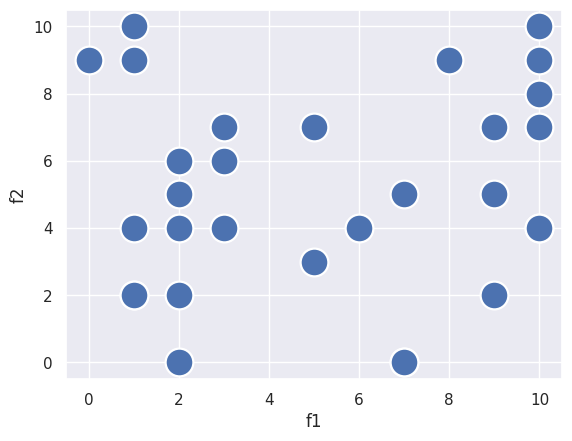
\includegraphics[scale=0.27]{img/diversity_all.png}
}
\hfill
\subfigure[Truncated selection of individuals based on $f^{(SO)}_{\texttt{DIV}}$.]{
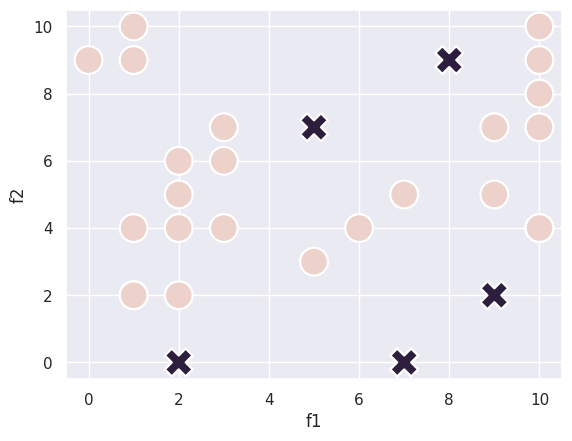
\includegraphics[scale=0.27]{img/diversity_so_selection.png}
}
\hfill
\subfigure[Selection of individuals using domination rank and $f^{(MO)}_{\texttt{DIV}}$ without the size component.]{
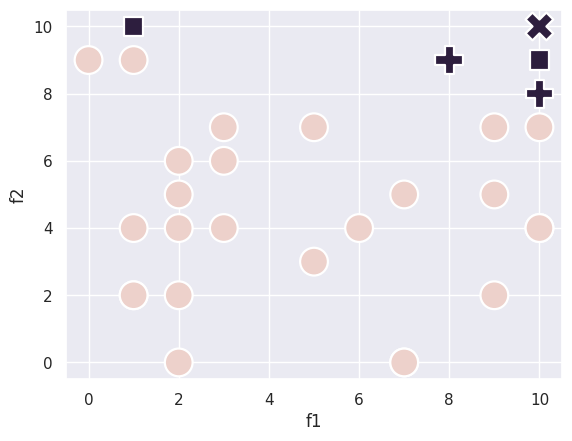
\includegraphics[scale=0.27]{img/diversity_mo_selection.png}
}

\caption{Illustration of different optimization criteria behavior in the diversity space.}
\label{fig:diversity}
\end{figure}

\subsubsection{\label{subsec:diversity-example}Differences in Diversity Nuance}

Grasping implications of the different diversity formulations
may prove tricky.
To help understand how the selection criteria and their respective formulations
impact the landscape of the search process, consider the example in \Cref{fig:diversity}.
Subfigure (a) shows a population of 30 points, the features of which
were each drawn from categorical uniform distributions.
In practice, the axes represent the number of language
features (statements, functions, etc.)
each individual (block) exhibits.
Within this space, the choice of modeling heuristic drastically affects
which blocks get selected to the next round of the algorithm.

Consider a scenario in which $f^{(SO)}_{\texttt{DIV}}$ is the fitness criterion,
and the algorithm uses a simple truncation selection method
to determine the survivors to the next generation.
In this case, the selection operator favors
blocks that are the farthest away
from any other blocks in the population, as subfigure (b) depicts.
The points depicted by black crosses are the ones
who survive the selection round.
While this mechanism does well to identify 
portions of the search space which the population
sparsely inhabits, it is prone to "forgetting"
areas of high density that do not contribute to the selection.
This issue resembles the problem of \textit{front degradation}
in traditional \Gls{MO} evolutionary computation.
The populaiton-wide retention mechanism of the \gls{SO} diversity
\gls{GA} seeks to combat this.

Alternatively, consider the \gls{MO} setting, in which
the algorithm carries out selection by means
of truncation based on the domination rank of the individual.
This combination of operators results in the selection depicted
in subfigure (c).
Points depicted in black are selected, and the shape of the point
depicts its domination rank.
Within this pure maximization framework, the problem makes itself apparent:
points depicting blocks that are larger drastically diminish the probability
of smaller blocks (mapped to the bottom-left quartile of the figure) propagating
to the next round of the algorithm.
It is for this reason that $f^{(MO)}_{\texttt{DIV}}$ contains a size component
that aims to circumvent this obstacle and allow for a more even
distribution of individuals.

Notably, only one selection overlaps between
the two selection mechanisms proposed here.
Within the scope of compiler testing, it is extremely difficult
to analytically reason about which
formulation is better suited for uncovering defects.
For this reason, we set out to empirically analyze both
formulations within this study.

\subsection{\label{subsec:proximity-ga}Semantic Proximity-Driven Search}

Syntactic analysis alone cannot paint a sufficiently
detailed picture for comparing blocks.
While effective as a means of measuring the structural composition of
blocks, the syntactic diversity criteria introduced in the previous
section fail capture the semantic nuances of generated code.
In this subsection, we introduce a slew of techniques culminating in two
complementary \gls{GA} formulations that seek to better
account for the indispensable semantic dimension of Kotlin code. 

\subsubsection{Modeling Semantic Proximity}

Strictly speaking, the mathematical requirements to effectively
measure the semantic similarity between two blocks
are the same as those that syntactic diversity requires:
a sound mapping from the domain of code, and a measure of distance
in the mapped space.
However, the multifaceted nature of Kotlin semantics
present difficulties that syntactic models do not face.
The \textsc{antlr4} \gls{CFG} implementation that the Kotlin
developer team supplies as part of the language specification
condenses the rules of the language in a structured and processable
manner.
This reduces the complexity of interpreting the syntactic similarity
of two blocks down to assessing their relation with respect to the grammar.
Unfortunately, no such construct exists for the semantic counterpart of Kotlin.

\newacronym{ML4SE}{ML4SE} {Machine Learning for Software Engineering}
\newacronym{ML}{ML} {Machine Learning}
\newacronym{NLP}{NLP} {Natural Language Processing}
\newacronym{NN}{NN} {Neural Network}

To address this problem, we turn to techniques used in the field
of \Gls{ML4SE}.
Ever since \citet{hindle2016naturalness} shared their findings on the
high regularity of code in 2016, the field of \gls{ML4SE} has experienced a boom
in popularity and development.
Crucially, the study suggested that software regularity 
emerging from a property the authors call \textit{naturalness}, as opposed to syntax.
Since then, researchers adapted, tuned, and extended techniques
at the intersection of \gls{ML} and \gls{NLP} and successfully applied
them at scale for common software engineering tasks.
Non-trivial chores previously exclusively reserved for developers could now
be at least in part automated at scale through new \gls{ML4SE} techniques.

Of particular interest to our research is a class of models
that use an internal numeric representation of pieces of code
to simultaneously model both the syntax and the semantics of the input.
These models largely rely on architectures revolving around a \gls{NN}
trained on one or more tasks, generally involving both code and natural language.
In \gls{NLP} research, the (lower-dimensional) numeric representation of token-represented
input is referred to as an \textit{embedding}.

Embeddings exhibit two key properties that make them suitable candidates for the goals
of our optimization framework.
Though impossible to interpret in isolation, embeddings retain
an interpretation of the textual representation fed into them.
We specifically select embedding mechanisms that have been trained
in an end-to-end fashion using multimodal training criteria, in the hope
of taking advantage of the generalizability of such approaches.
Second, by populating a space with the embeddings of Kotlin code,
the notion of \textit{proximity} can simply be expressed by means
of a distance metric in the projected domain.

\begin{figure}[t]
\vspace{2cm}
\centering
\begin{tikzpicture}[transform canvas={scale=1.0},node/.style={circle, draw, thick}]

\foreach \Z in {0,0.5,1,1.5}
 {\draw[fill=gray,draw=black] (-8,0,\Z) rectangle (-7.25,1,\Z);}

\node[] at (-7.5,1.5)   (a) {Chromosome};

 \draw [-stealth] (-7.15, 0.5) -- node[pos=0.5,above]{Construct} (-5.5, 0.5);
 
 \pgfmathsetmacro{\cubex}{1.25}
\pgfmathsetmacro{\cubey}{1.25}
\pgfmathsetmacro{\cubez}{1.25}
\draw[black,fill=gray] (-4,1,0) -- ++(-\cubex,0,0) -- ++(0,-\cubey,0) -- ++(\cubex,0,0) -- cycle;
\draw[black,fill=gray] (-4,1,0) -- ++(0,0,-\cubez) -- ++(0,-\cubey,0) -- ++(0,0,\cubez) --  cycle;
\draw[black,fill=gray] (-4,1,0) -- ++(-\cubex,0,0) -- ++(0,0,-\cubez) -- ++(\cubex,0,0) -- cycle;

\node[] at (-4.25,1.875)   (a) {Text};

\draw [-stealth] (-3.25, 0.5) -- node[pos=0.5,above]{NN Input} (-1.75, 0.5);

  \foreach \y in {1,...,3}{
      \node[node] (i\y) at (-1,\nodesep*\y-0.5) {};
      \node[node, right=\layersep of i\y] (h1\y) {};
      \node[node, right=\layersep of h1\y] (h2\y) {};
    }

  \foreach \source in {1,...,3}
  \foreach \dest in {1,...,3}{
      \path[-stealth, thick] (i\source) edge (h1\dest);
      \path[-stealth, thick] (h1\source) edge (h2\dest);
    }

\draw[] (-1.5, -0.5) rectangle (1.25, 1.5);

\node[] at (-0.125,1.875)   (a) {Embedding NN};

\draw [-stealth] (1.5, 0.5) -- node[pos=0.5,above]{NN Output} (3.5, 0.5);

\node[right,scale=0.9] at (3.5,0.5)
    {$\begin{pmatrix}
        0.4\\[0.3em]
        0.2\\
        \vdots \\
        0.7
       \end{pmatrix} \in \mathbb{R}^{k}$};
      
%\draw [-stealth] (4.25, 0.25) -- (5.5, 0.25) -- (5.5,-0.45);


  \def\rvec{.8}
  \def\thetavec{30}
  \def\phivec{60}
  
  \draw[-stealth] (4.75, -0) -- (6.5, -0);
  
  % AXES
  \coordinate (O) at (8,-0,0);
  \draw[thick,->] (7,-0,0) -- (8,0,0) node[below left=-0.5]{$x$};
  \draw[thick,->] (7,-0,0) -- (7,1,0) node[right=-0.5]{$y$};
  \draw[thick,->] (7,-0,0) -- (7,0,1) node[above=-0.5]{$z$};
  
  \filldraw[gray2] (7.5,1, 0.5) circle (2pt) node[anchor=west]{$b_1$};
  \filldraw[gray2] (7.35,0.5, 0.5) circle (2pt) node[anchor=west]{$b_2$};
  \filldraw[gray2] (7.75,0.75, 0.5) circle (2pt) node[anchor=west]{$b_3$};
  
  \filldraw[gray1] (7,-0.5, 0) circle (2pt) node[anchor=west]{$b_4$};
  \filldraw[gray1] (7.35,0, 0.5) circle (2pt) node[anchor=west]{$b_5$};
  \filldraw[gray1] (7.85,-0.1, 0.5) circle (2pt) node[anchor=west]{$b_6$};
  
  \filldraw[red] (6.75,0.5, 0.5) circle (2pt) node[anchor=south]{$b_7$};
\end{tikzpicture}
\vspace{0.5cm}
\caption{Visualization of the code embedding process.}
\label{fig:embeddings}
\end{figure}

\Cref{fig:embeddings} contains an illustration of the embedding pipeline.
To compute the proximity of two chromosomes during search,
we first convert the ordered snippet list into the
Kotlin code, without retaining any additional information.
We then feed the code as input to the embedding \gls{NN} of choice,
and retrieve the real-valued vector it computes as output.
By caching previously computed blocks, the topology
of a projected space emerges, and the similarity of two blocks
is measured in terms of their proximity (distance).
The points depicted in the coordinate system on the right
of \Cref{fig:embeddings} are color-coded to highlight their
proximity within the space.
Blocks corresponding to points $b_1, b_2$, and $b_3$ all
are in close proximity to one another, as are the blocks
pertaining to $b_4, b_5$, and $b_6$. 
$b_7$ is farther apart, denoting its dissimilarity to either cluster.

\subsubsection{Selecting Proximity Targets}

To completely integrate the notion of semantic proximity 
in our \gls{GA}, we require a notion of individual fitness.
The notion of diversity proposed in the previous section is a candidate 
for this purpose, however, it suffers from two notable drawbacks.
First, embedding \gls{NN}s operate on the entire textual representation
of the code, which means that (unlike our syntactic formulation)
information such as randomly generated
identifier names influences the embedding of the chromosome.
In practice, this means that input is likely to be noisy, artificially
affecting diversity estimates.
Second, embeddings of current code models tend to have a 
relatively high number of dimensions, and relatively small numerical values
at each position.
This does not bode well with our population-adaptive
diversity heuristic, which attempts to simultaneously consider all dimensions
in a scalarization of the distance metric.

As an alternative, we propose a heuristic which seeks to \textit{maximize the proximity}
between the population of a \gls{GA} and a \textit{static} collection of \textit{target}
pieces of Kotlin code.
Intuitively, this approach seeks to generate code that is \textit{as close as possible}
to a pre-defined set of targets.
Naturally, we must ensure that a suitable collection of code serve as targets during optimization.
For this purpose, we turn our attention to a collection of test inputs that contributors
to the Kotlin put together with the goal of verifying a broad range of
compiler and language features.
These inputs are publicly available as part of the Kotlin repository
\footnote{https://github.com/JetBrains/kotlin/tree/master/compiler/testData}.

The proximity optimization concept rests upon two core assumptions.
The first assumption is that
the set of targets provided to the algorithm consists of "\textit{interesting}"
test cases for the compiler.
By interesting, we refer both to the relevancy of the test cases
to the broader scope of the language, as well as the behavior they
cause during compilation.
Since the data set we use by default has been curated by
compiler developers over a long period
of time, we have no reason to doubt the validity of this assumption.
Second, we assume that within the embedding space, projections
that are close to \textit{interesting} test cases are likely to be, themselves,
\textit{interesting}.
On the surface, this is a reasonable proposition: pieces of code
that are similar to hand-crafted compiler test cases
may well trigger compiler edge case behavior that
the static test misses.
However, the practical implications of this assumption
heavily depend on the choice of similarity metric.

To ensure that the mapping to the embedding space appropriately
shapes the output domain, we must carefully choose a model
that has shown good performance on multiple code-centric tasks.
To our knowledge, there are currently no available open-source models
that have either been pre-trained or fine-tuned for Kotlin-specific
tasks and thoroughly evaluated in an empirical study.
With this in mind, we select \textsc{CodeBERT} \cite{feng2020codebert}
as the default option for the remainder of this study.
\textsc{CodeBERT} is a Transformer-based \cite{vaswani2017attention} model
that has been pre-trained on a large corpus
of open-source repositories containing several languages.
Though Kotlin is not part of \textsc{CodeBERT} training set,
its closest relative, Java, is.
Furthermore, the architects of the \textsc{CodeXGLUE} \cite{lu2021codexglue}
, a popular \gls{ML} for code-related tasks dataset,
 have selected \textsc{CodeBERT} as the default
benchmark to compare against in several categories, attesting to
its generalizability.

Finally, to better assess the performance of the algorithm,
some degree of interpretability is required.
The data set of tests provided in the Kotlin repository
is vast, encompassing over 19,000 files
organized in almost 2,000 directories.
To parse the result of our fuzzers with respect
to this extensive dataset, we reduced the number of
selected targets by means of clustering.
We empirically assessed several clustering algorithms
provide sensible default options based on how well
the clusters reflect the original directory structure.

\subsubsection{Single-Target Proximity Optimization}

\begin{algorithm}[t]

	\SetKwData{Left}{left}
	\SetKwData{This}{this}
	\SetKwData{Up}{up}
	\SetKwFunction{init}{InitializeAndEvaluatePopulation}
	\SetKwFunction{terminate}{ShouldTermiante}
	\SetKwFunction{offspring}{CreateAndEvaluateOffspring}
	\SetKwFunction{select}{SelectIndividuals}
	\SetKwFunction{time}{TimeElapsed}
	\SetKwFunction{process}{ChooseBestForEachTarget}
	\SetKwFunction{clone}{Clone}
	\SetKwFunction{best}{BestBlockForEachTarget}
	\SetKwFunction{sample}{Sample}
	\SetKwInOut{Input}{Input}
	\SetKwFunction{shuffle}{Shuffle}
	\SetKwInOut{Output}{Output}
	\Input{Target Set $\mathcal{T}$, Population size $n$, Node to sample $\mathcal{N}$, Context $\mathcal{C}$, Time Budget $s$, Target Time Budget $s_t$}
	\Output{Collection of generated Kotlin files}
	\BlankLine
	\DontPrintSemicolon
	\shuffle{$\mathcal{T}$}\;
	$i \leftarrow 1$\;
	\While{$\neg$ \time{$s$}}{
	$T \leftarrow \mathcal{T}_i$\;
	$t \leftarrow 1$\;
	$P_1 \leftarrow $ \init{$n, \mathcal{N}, \mathcal{C}$}\;
		\While {$\neg$ \time{$s_t$}}{
		\process{$P_t, \mathcal{T}$}\;
		$O_t \leftarrow$ \offspring {$P_t$}\;
		$P_{t+1} \leftarrow$ \select{$P_{t}, O_{t}, f^{(SO)}_{\texttt{PRO}}$}\;
		$t \leftarrow t + 1$\;
		}
		$i \leftarrow i + 1$\;
	}
	\Return \best{$\mathcal{T}$}\;
	\caption{Single-Target Proximity Genetic Algorithm}
	\label{alg:stpga}
\end{algorithm}

To tie our proximity formulation together, we first propose an algorithm
that iteratively attempts to minimize the distance to
each of the targets in the data set.
This follows the paradigm that \citet{tonella2004evolutionary} established
in one of the earliest successful applications of \gls{GA}s
to the task of automated unit test generation.
The function to optimize is given by a particular selected
target, and measures the distance from the individual to that target.
\Cref{eq:proximity_so} gives the definition of this \gls{SO}
objective, with $b$ the block to a evaluate, $t_i$ a target that the
algorithm is attempting to reach, $d$ a measure of distance,
and $e$ an embedding function as described in the previous
subsection.
\Cref{alg:stpga} illustrates  the pseudocode of the entire procedure.

\begin{equation}
\min_{b \in \mathcal{B}} f^{(SO)}_{\texttt{PRO}}(b, t_i) = d(e(b), t_i)
\label{eq:proximity_so}
\end{equation}

The algorithm is structured in two nested loops.
Before iterations start, the algorithm first shuffles
the 
The outer loop first selects a target (line 4),
before attempting to optimize a random population towards that target,
in a nested loop that applies a \gls{GA} (lines 5-11).
In addition to running the nested \gls{GA},
each inner iteration also considers whether the current population has
contains better improvements with regard to \textit{any}
target in the data set, not just the one being optimized.
This information does not affect selection -  the scope of this
additional step (line 8) is to avoid discarding individuals
that would have been closest to \textit{some} target.
The algorithm returns a set of blocks that are closest to at least one target.

\subsubsection{Many-Objective Proximity Optimization}

To complement the iterative \gls{SO} formulation, we also propose
an \gls{MO} alternative that attempts to simultaneously minimize the distance
to each target in the data set.
Compared to the previous alternative, the \gls{MO} option could provide a
more comprehensive overview of the search landscape by also
selecting blocks which are not necessarily \textit{closest}
to any one target, but relatively close to multiple targets at the same time.
The \gls{MO} fitness function underlying the optimizaiton method
is given by \Cref{eq:proximity_mo}.


\begin{equation}
\min_{b \in \mathcal{B}} f^{(MO)}_{\texttt{PRO}}(b, \mathcal{T}) = \left\lbrace d(e(b), t_i)|~t_i \in \mathcal{T} \right\rbrace
\label{eq:proximity_mo}
\end{equation}

The pseudocode of the algorithm is analogous to that of \Cref{alg:modga}, 
except selection and archival are carried out based on $f^{(MO)}_{\texttt{PRO}}$
rather than its diversity counterpart.
Of note is that the number of individual objectives is generally
much higher for the proximity formulation.
This is because the number of individual language that the fuzzer supports
is relatively limited, whereas the number of available test cases, even
when reduced by clustering, is much higher.
This warrants the use of standard techniques for bounding the elitist archive, such
as discretization or pruning.
Alternatively, a user could also configure the \gls{GA} to use a lower population size.

\subsubsection{Scalarization-Based Proximity Optimization}

\newacronym{WS}{WS}{Whole-Suite}

The final proximity-centered formulation we propose finds its roots
in the \gls{WS} approach put forward by \citet{fraser2012whole}.
This approach follows the common \gls{GA} framework explored in this
thesis, with one key exception.
Individuals in the \gls{WS} approach are \textit{test suites},
which constitute unordered collections of lower-level
test individuals.
In our case, each suite $S$ is a group of blocks.
To evaluate a suite, \gls{WS} performs a technique called
\textit{scalarization} \cite{deb2013multi}, which translates
the \gls{MO} problem down to an \gls{SO} counterpart.
\Cref{eq:proximity_ws} encapsulates the fitness this approach
is based on, with each suite $S$ having a fitness based on the sum
of smallest distances between the blocks in $S$ and each target $t$.

\begin{equation}
\min_{b \in \mathcal{B}} f^{(SO)}_{\texttt{WS}}(S, \mathcal{T}) = \sum_{t \in \mathcal{T}} \min_{b^{(i)} \in S} d(e(b^{(i)}), t)
\label{eq:proximity_ws}
\end{equation}

We incorporate $f^{(SO)}_{\texttt{WS}}(S, \mathcal{T})$ in a \gls{GA} nearly identical to
\Cref{alg:sga}.
However, unlike all previous formulations, \gls{WS} performs variation and selection
at the suite-level, rather than on individual blocks.
Mutation operators include addition, removal, and swapping of individual blocks,
while recombination simply swaps blocks between two separate test suites.
Finally, we note that \gls{WS} has several known limitations, including that
it can fail to retain individually valuable blocks.
This shortcoming emerges as a consequence of the scope
of the variation and selection operators, neither of which
attempts to retain individual components of the suite.
Newer approaches like \textsc{DynaMOSA} have demonstrated increased performance
relative to \gls{WS}, however, the simplicity of the \gls{WS} approach
makes it a better candidate for studying and interpreting the effects of operating
at a larger level than blocks.

%\subsection{\label{subsec:compiler-ga} Compiler Integration}
\chapter{\label{cha:tool}Tool}
\chapter{\label{cha:study}Empirical Study}

This chapter outlines the empirical evaluation we carried out
to evaluate the prototype implementation of \kf~ its six
constituent search algorithms.
\Cref{sec:subjects} begins by establishing the algorithms
we set out to assess within this study, and \Cref{sec:rqs} fixates the research
questions we aim to answer.
\Cref{sec:metrics} establishes the metrics we use to determine the
performance and behavior of each algorithm.
Lastly, \Cref{sec:protocol} details the experimental protocol
we follow to obtain concrete results.

\section{\label{sec:subjects}Evaluation Subjects}

\newacronym{SODGA}{SODGA}{Single-Objective Diversity Genetic Algorithm}
\newacronym{MODGA}{MODGA}{Many-Objective Diversity Genetic Algorithm}
\newacronym{STPGA}{STPGA}{Single-Target Proximity Genetic Algorithm}
\newacronym{MOPGA}{MOPGA}{Many-Objective Proximity Genetic Algorithm}
\newacronym{WSPGA}{WSPGA}{Whole-Suite Proximity Genetic Algorithm}

To gather a comprehensive overview of the performance, behavior,
and implications of the approaches proposed in \Cref{cha:algorithm},
we evaluate six prototype implementations, split between three distinct categories.
The first category contains a single algorithm, \gls{RS},
introduced in \Cref{subsec:random-sampling}.
The second class contains two instances of syntactic-oriented
algorithms: \gls{SODGA} and \gls{MODGA}, based on the formulations
proposed in \Cref{subsec:diversity-ga}.
The final group of algorithms focuses on the semantic proximity
formulations detailed in \Cref{subsec:proximity-ga}, and contains three instances.
\gls{STPGA}, \gls{MOPGA}, and \gls{WSPGA}
implement the three proposed approaches.

\Cref{tab:algs} contains an overview of the six implemented algorithms.
\gls{SODGA}, \gls{STPGA}, \gls{WSPGA} behave like \gls{SO} algorithms
(though \gls{STPGA} repeatedly switches objectives),
while \gls{MODGA} and \gls{MOPGA} implement \gls{MO} formulations.
We opt for the use of tournament selection for \gls{SO} scenarios, and
domination rank counterparts for \gls{MO} instances.
For \gls{GA}-based algorithms, we turn to established literature values
to determine the size of the population and further selection details.
However, applications of evolutionary fuzzing to
compiler testing are scarce, and established evolutionary fuzzing
tools like \textsc{VUzzer} \cite{rawat2017vuzzer} and
\textsc{V-Fuzz} \cite{li2019v} make no recommendation in these regards.

As such, we turn to standard values used in software
testing literature, particularly of \textsc{EvoSuite}, which uses
a population size of 50 and a tournament size of 10
\cite{fraser2011evosuite, panichella2017automated}.
Past research by \citet{arcuri2013parameter}
has shown that default values can provide solid
performance in a broad set of scenarios, in the context of software testing.
Though these findings provide no guarantees for the task of compiler
testing in particular, we believe these are sensible
starting points that circumvent the expensive requirements of parameter
tuning over all proposed algorithms.

\begin{table}[]
    \centering
    \begin{tabular}{cccc}
    % \toprule
    Heuristic & Fitness & \# Objectives & Selection \\
    \midrule
    \gls{RS} & - & - & - \\
    \midrule
    \gls{SODGA} & $f^{(SO)}_{\texttt{DIV}}(b, P) = \frac{1}{1 + dis(b, P)}$
    & 1 & Tournament\\
    \midrule
    \gls{MODGA} & $f^{(MO)}_{\texttt{DIV}}(b) = \left\lbrace -f_{sz}(b), ~f_{l_i}(b)|~l_i \in \mathbb{L}
    \right\rbrace$ & $\mid \mathbb{L} \mid + 1 = 6$ & Dom. Rank, Tournament\\
    \midrule
    \gls{STPGA} & $f^{(SO)}_{\texttt{PRO}}(b, t_i) = d(e(b), t_i)$ & 1, adaptive & Tournament\\
    \midrule
    \gls{MOPGA} & $f^{(MO)}_{\texttt{PRO}}(b, \mathcal{T}) =
    \left\lbrace d(e(b), t_i)|~t_i \in \mathcal{T} \right\rbrace$ & $\mid \mathcal{T} \mid$ & Dom. Rank, Tournament\\
    \midrule
    \gls{WSPGA} & $f^{(SO)}_{\texttt{WS}}(S, \mathcal{T}) =
    \sum_{t \in \mathcal{T}} \min_{b^{(i)} \in S} d(e(b^{(i)}), t)$ & 1 & Suite Tournament\\
    \bottomrule
    \end{tabular}
    \caption{Overview of evaluated algorithms.}
    \label{tab:algs}
\end{table}

\section{\label{sec:rqs}Research Questions}

The empirical analysis of the proposed approach aims to answer the following
research questions, which we reiterate from \Cref{sec:aim}:

\begin{quote}
\centering 
\emph{\textbf{RQ1:} How do meta-heuristic guidance
criteria influence the properties of test programs
generated by fuzzing?}
\end{quote}

To better differentiate between the six proposed approaches and their
individual most significant guiding parameters, we split the \textit{RQ1}
into three subquestions:

\begin{quote}
\centering 
\emph{\textbf{RQ1.1:} How does the simplicity bias
impact the properties of files generated by \gls{RS}?}
\end{quote}

\begin{quote}
\centering 
\emph{\textbf{RQ1.2:} How does the projection space
topology influence the properties of files generated
by syntactic diversity-driven heuristics?}
\end{quote}

\begin{quote}
\centering 
\emph{\textbf{RQ1.3:} How does target selection
influence the properties of files generated
by semantic proximity-driven heuristics?}
\end{quote}

The three subquestions address each of three generative
heuristic categories by tuning their core elements.
For \gls{RS}, by far the most influential hyperaparameter is
the simplicity bias, which governs both the structure and complexity of generate expressions.
For diversity heuristics, the manner in which diversity is computed drives the selection procedure.
Finally, the number of targets that proximity-heuristics receive is crucial for their search process.
Once established, the most sensible settings revealed by the previous subquestions can be used
to empirically assess the performance of each category of algorithms in comparison to the others,
as stated in \textit{RQ2}:

\begin{quote}
\centering 
\emph{\textbf{RQ2:} How do the random search, syntactic
diversity, and semantic proximity generative heuristics
perform in terms of uncovering bugs in the Kotlin compiler?}
\end{quote}

To answer the second research question, we seek to measure
the performance of the best algorithm from each class and compare
both their bug-finding capabilities and efficiency.

\section{\label{sec:metrics}Evaluation Metrics}

To measure the performance of our algorithms, we focus on the two
dimensions of \textit{effectiveness} and \textit{efficiency}.
Before addressing those measures, however, we first establish
the meaning of a compiler defect within the framework
of \gls{DT}.
For the purposes of this study, a generated piece of Kotlin code
$b$ passes through two versions of the compiler,
\texttt{K1} and \texttt{K2}.
$b$ is said to have uncovered a deffect if either of following cases occurs:

\begin{enumerate}
    \item \texttt{K1} successfully compiles $b$ and \texttt{K2} does not.
    \item \texttt{K1} compiles $b$ and \texttt{K2} crashes.
    \item \texttt{K2} successfully compiles $b$ and \texttt{K1} does not.
    \item \texttt{K2} compiles $b$ and \texttt{K1} crashes.
    \item \texttt{K1} and \texttt{K2} both crash.
\end{enumerate}

In the above listing, we define a \textit{successful} compilation
as one that results in an output object
(for our purposes, a \texttt{jar} file).
An unsuccessful compilation is one that \textit{completes}, but
does not result in an output object (i.e., the compiler
has detected that the code is erroneous).
A \textit{crash} occurs when compilation fails to complete altogether.
\Cref{tab:defects} contains a visualization of the types of defects
that can emerge during a differential testing round.

Only two types of behaviors are considered considered correct within
this system: either both systems successfully compile an input
file to a \texttt{jar} object, or both fail to do so, without crashing.
In any other case, we consider the behavior erroneous and attach it a 
label that categorizes the defect according to the list above.
Since the tangible goal of this study is to help improve
the quality of the \texttt{K2} compiler, we only focus on error types
that break backwards compatibility (I and III), or that cause \texttt{K2}
to crash (IV and V).
We emphasize errors that only cause defects in \texttt{K1} (type II)
less than their counterparts, as this version is to be replaced in the future.

\begin{table}[]
    \centering
    \begin{tabular}{cc|ccc}
        &&\multicolumn{3}{c}{\texttt{K1} outcome}\\
        &&Success & Failure & Crash\\
        \midrule
        \parbox[t]{2mm}{\multirow{3}{*}{\rotatebox[origin=c]{90}{\texttt{K2} outcome}}}& Success & \ding{52} & Type I & Type II \\
        & Failure & Type III & \ding{52} & Type II\\
        & Crash & Type IV & Type IV & Type V\\
    \end{tabular}
    \caption{Types of compiler defects.}
    \label{tab:defects}
\end{table}

\newacronym{AUC}{AUC}{Area-Under-Curve}

We use this notion of defects to measure the
performance of the six proposed algorithms.
The effectiveness of a fuzzer run is the number
of files generated within that run that cause any defects (types I-V)
after differential testing.
This metric captures the performance of the fuzzer after the exhaustion,
however, an additional measure of efficiency is required to underline
an algorithm's behavior over time.
To this end, we express the efficiency of a run through the
\gls{AUC} metric.

Informally, when running a fuzzer algorithm, snapshots of its performance
can be expressed as 2-dimensional points, where the $x$ axis represents the time elapsed,
and the $y$ axis, the number of uncovered defects.
After several snapshots have been taken at approximately comparable
times for multiple algorithms, the curve that emerges from connecting the points
corresponding to snapshots splits the space in two.
The area under this curve provides a means of comparing how quickly
algorithms uncover bugs.
Given a set $P$ of two dimensional points $p_i$, with $p_i^{(1)}$
the time at which the snapshot was taken and $p_i^{(2)}$ the number of defects
uncovered by generated files until that point,
we compute the \gls{AUC} according to the trapezoidal rule approximation
given by \Cref{eq:auc}.

\begin{equation}
    \frac{\sum_{i=1}^{\mid P \mid - 1} \Large( p_i^{(2)} + p_{i + 1}^{(2)} \Large)
\cdot (p_{i + 1}^{(1)} - p_{i}^{(1)})}{p_{\mid P \mid}^{(1)} - p_1^{(1)}}
\label{eq:auc}
\end{equation}

\section{\label{sec:protocol}Experimental Protocol}

To ensure the robustness of the empirical evaluation, we perform repeated runs
to determine the relative performance of the six proposed methods.
Due to the large number of possible hyperparameter and heuristic
combinations, as well as the large quantity of computational resources
required to perform \gls{DT} on generated files, we focus these
techniques on performance evaluations.
To determine appropriate parameter ranges for variables not explored in previous work,
we rely on fewer, longer runs, instead.

\subsubsection{Statistical Analysis}

Where appropriate, we additionally perform statistical tests in accordance
with standard practices related to empirical analysis of
randomized software engineering algorithms \cite{arcuri2014hitchhiker}.
We employ the paired-data version of the
Wilcoxon \cite{conover1999practical} signed-rank test to verify
whether the performance (either efficiency or effectiveness) of one algorithm
differs from that of another.
This test operates on a null hypothesis that the distribution
of the difference between two sample populations is symmetric around a mean of 0.
Informally, the main consequence of the alternative hypothesis is that
there is a significant difference between the measurements emerging from the 
two algorithms subject to comparison.
The $p$-value computed by this test determines whether the evidence
supports the null or the alternative hypothesis.
\textit{Significant} $p$-values ($<$ 0.05) imply a high probability of the latter being true.

To measure the how much the performance of two
algorithms differs in favor of either one, we use the method
established by \citet{vargha2000critique} $A_{12}$ for computing the \textit{effect size}
of a population of samples.
The $A_{12}$ captures the stochastic difference between the 
distributions approximated by the two populations and, with respect
to our study, shows which distribution skews higher based on evidence from
several runs.
An $A_{12}$ measurement of $0.5$ in a comparison between two 
algorithms $a_1$ and $a_2$ denotes the two approaches
are equivalent.
Higher values favor $a_2$, while, symmetrically, lower values favor $a_1$.

\subsubsection{Experiment Length and Heuristic}

To understand how the simplicity bias influences the nature
of generated files (\textit{RQ1.1}), we test several values of this parameter under
the setting of \gls{RS}.
Random Sampling is a prime candidate for uncovering the effects of this
option, as there are very few external factors that could otherwise alter
the shape of block generation.
We experiment simplicity bias values of between 0.4 and 0.6, as we empirically found
that values outside this range either lead to blocks too large to scale in
more sophisticated search heuristics, or too small to build a sufficiently
complex context.
We run \kf~ using \gls{RS} for 90 minutes for each setting of simplicity bias.

To answer \textit{RQ1.2}, we perform two 90-minute runs for both \gls{SODGA} and \gls{MODGA}:
one with a Euclidean norm distance measure ($d(e(b_1), e(b_2)) =
\sum_{1 \leq i \leq \mid e(b_{\{1,2\}}) \mid} \sqrt{(b_1^{(i)} - b_2^{(i)}}$),
and one with an $l^\infty$ norm equivalent ($d(e(b_1), e(b_2)) =
\max_{1 \leq i \leq \mid e(b_{\{1,2\}}) \mid} \mid b_1^{(i)} - b_2^{(i)} \mid$.
The results would help uncover how a more stringent measures of diversity
influences the quality of the generated files.
Next, we attempt to answer \textit{RQ1.3} by varying the number of targets provided
to \gls{STPGA}, \gls{MOPGA}, and \gls{WSPGA} between 50 and 200, which
helps understand how the number of objectives affects
the generative process.
Finally, we answer \textit{RQ2} by considering the effectiveness and efficiency
of \gls{RS}, and the two most sensible approaches that emerge from the analysis of the
previous subquestions.

\subsubsection{Experimental Environment}

We carry out all \gls{DT} procedures through the publicly released
Kotlin version \texttt{1.8.20-RC-release-288}
\footnote{https://github.com/JetBrains/kotlin/releases/tag/v1.8.20}.
We ran all generation, \gls{DT}, and analysis experiments on a
AMD Ryzen 7 5800H machine, running on the Manjaro Talos 22.1.2
\gls{OS}, with 16 gigabytes of RAM.
We executed all experiments in isolated containers using Docker.

We ran 5 instances of \gls{RS} to answer \textit{RQ1.1}.
Three runs \gls{SODGA} and \gls{MODGA} provide the data for \textit{RQ1.2},
while four runs for each of the three proximity algorithms constitute the experimental
analysis for \textit{RQ1.3}.
We additionally executed 10 runs each for each of the most promising algorithm
from each class to answer \textit{RQ2},
for a total of $5 + 3 + 12 + 3 \times 10 = 50$ total fuzzing sessions.
We additionally perform one other long-term (82 hour) fuzzing campaign to
gain insight into the scale-related behavior and limitations of the fuzzer.
\chapter{\label{cha:results}Results}

The aim of this thesis is to gain insight into the behavior and applicability
of heuristics to task of differential testing of the Kotlin compiler.
To achieve this goal, this chapter seeks to answer the research questions posed in
\Cref{sec:rqs} through empirical evidence and statistical analysis.
We structure the analysis of the results as to mirror the hierarchy
of research questions.
\Cref{sec:resrq1} analyzes the effect of the the most impactful
hyperparameters and the ramifications on the generative heuristics.
\Cref{sec:resrq2} details the performance of the best representative
of each heuristic category.

\section{\label{sec:resrq1}Influence of Guidance Parameters}

We begin our analysis of hyperparameter influence by considering the effects of
the simplicity bias on the structure, size, and number of files that \kf~ generates
in \Cref{subsec:simpl_bias}, followed by the effects of distance metrics on diversity
heuristics in \Cref{subsec:distance_effect}, and finally the impact 
of target selection in \Cref{subsec:targets_effect}.

\subsection{\label{subsec:simpl_bias}Effects of Simplicity Bias on Random Sampling}

To study the effects of the simplicity bias, we focus on the size and number of files
generated by \gls{RS}.

\subsection{\label{subsec:distance_effect}Effects of Distance Metric on Syntactic Diversity-Driven Search}

\subsection{\label{subsec:targets_effect}Effects of Target Set on Semantic Proximity-Driven Search}


\section{\label{sec:resrq2}Performance of Heuristics}
\addcontentsline{toc}{part}{Part III}
\chapter{\label{cha:discussion}Discussion}

This section discusses the totality of the study and contextualizes
potential implications.
We begin by analyzing the limitations of our approach in \Cref{sec:limits},
before addressing potential threats to the validity of the research in \Cref{sec:threats}.
\Cref{sec:future} provides recommendations regarding potential 
avenues of future expansion of this study.

\section{\label{sec:limits}Limitations}

Throughout this study, we generated, compiled, and analyzed
roughly 200,000 Kotlin files, and uncovered five categories
of defects affecting three components of the Kotlin compiler.
The Kotlin compiler team verified all of these errors and is
working on targeted fixes for several of them.
In this process, several non-trivial
underlying biases and restraints that
\kf~carries came to light.
In this section, we analyze both the practical and theoretical
limitations of the fuzzer, critically assess them, and propose solutions.

\paragraph{Language Features}
The set of language features that the fuzzer currently supports is limited
to functions, four types of expressions, and statements.
This limitation, which we imposed to ensure the feasibility of the study,
drastically limits the domain of code that \kf~can generate.
In practice, this restriction means that any defects that are related to core language features,
such as classes, are outside the reach of the current research prototype.
Extending the set of language features is paramount for enhancing
the practicality of the tool and for effectively exploring the Kotlin syntax.
In its current state, extending novel language features consists of simply
implementing either one or two additional Java classes and making them accessible
in parent \gls{CFG} nodes.

\paragraph{Context}
Throughout the study, the root context used for sampling
consisted of a limited collection of standard library files mostly containing exceptions,
throwables, as well as numeric, logical, and string types.
Besides severely limiting the number of objects and classes
that \kf~ can generate, this factor also affects the
set of language features that our tool can leverage.
For instance, \texttt{for} statements in Kotlin can only be applied
to constructs that implement specific methods, also known as \textit{container} classes.
In the current context, no such type is available, further limiting the syntax \kf~can leverage.

\paragraph{Generative Constraints}
To ensure the validity of generated code, we embed
numerous constraints and biases in the sampling process.
The implementation of these constraints has proven effective,
as all sampled code examined in this study was valid (i.e., either \texttt{K1} or \texttt{K2}
compiled the code, unless a \texttt{OOM} error occurred).
However, these constraints may drastically reduce the domain of code that \kf~ can generate,
thus possibly also missing out on additional defects.
For instance, constraints such as \textit{the return type of a function must be samplable in the current context}
may render much of the context useless.
While intuitively respecting such a constraint is sensible
(if there is no way to sample a type in the current context, it is impossible to write a function
that returns such a type), it could be that breaking this constraint
might lead to false negative defects.
The genetic recombination proves this by breaking one such constraint, which
lead to the nested function defect discussed in \Cref{sec:buganalysis}.
Exploring how generative constraints affect the quality of the generated code and whether
they lead to additional defects requires careful and incremental changes, that we do not cover in this study.

\paragraph{Representation and Genetic Operators}
The hierarchical \textit{fragment, snippet, block} representation
is sufficient to meaningfully separate code
based on complexity and scope, but lacks the precision needed to
explore certain corner cases.
For instance, neither snippets, nor blocks are recursive,
which means variation operators in \gls{GA} algorithms
are only able to operate on the highest scope
of the file.
This limitation leaves out numerous cases in which
code can be exchanged on smaller levels, in turn exploring a new dimension of the language.
A representation capable of capturing this level of detail
requires a recursive implementation of blocks and fragments,
the foundation of which is already implemented in the current implementation of \kf.

\paragraph{\gls{GA} Convergence}
The application of \gls{GA}-based formulations to fuzzing
raises the problem of convergence.
Especially visible in the cases of \gls{SODGA} and \gls{STPGA},
the problem stems from the fact that relatively stable sets of solutions
may emerge quickly in those \gls{GA}s.
Since longer fuzzing campaigns become wasteful and redundant in those
scenarios, a mechanism that breaks this stability would enable
longer fuzzing runs.
Two options to alleviate this problem include restart mechanisms to effectively reset the search process,
and altering the targets of proximity-based algorithms.

\section{\label{sec:threats}Threats to Validity and Reproducibility}

Threats to \textit{construct validity} stem from the connection between 
the practical measures employed to quantify theoretical aspects of the study.
In this regard, we use standard \gls{DT} procedures to quantify
compiler defects, and link uncovered defects to static, measurable properties of
the generated code.
We also employ common metrics of effectiveness and efficiency that
are standard practice throughout empirical software engineering research.

Threats to \textit{internal validity} regard factors that could lead
to confounding the causes of observed phenomena.
We take several measures to address the large degree of randomness
inherent to fuzzing approaches.
First, we individually assess each uncovered defect
and analyze the components of the fuzzer involved in its generation.
Second, we ensure the fairness of
the comparisons by sharing parameters
between different configurations with
default values from literature, where available.
We also perform the comparison using a single implementation
of the tool, that relies on the same sampling process and genetic operators.
Lastly, to assess the effectiveness and efficiency of our algorithms,
we repeat independent runs 10 times, and report average values
that are subject to standard statistical analyses.

Threats to \textit{conclusion validity} affect the relation between the available data
and the credibility of the conclusions we derive based on it.
To this end, we base our analysis on over 200,000 generated files,
and vary the essential hyperparameters of our algorithms to several
sensible values.
We additionally perform statistical tests to compare algorithms representative
of their respective class.
In particular, we base our performance conclusions on
the application of the Wilcoxon signed-rank test, which
is a statistical procedure that does not make any assumptions
about the distribution of the underlying data.

Threats to \textit{reproducibility} concern factors that might cause the application
of the same research methods to result in significantly divergent or conflicting observations.
To mitigate this, we supply the entire code base that implements \kf~ \footnote{TODO, not available in draft},
in addition to the entire set of generated files, adjacent preprocessed data, and analytics tools \footnote{TODO}.
We also provide extensive documentation regarding our research methods (within this study),
as well regarding our tool, its configuration, and its applicability.
To ensure that no environmental factors interfere with the fuzzer,
we use containerization to isolate the dependency management and runtime of \kf.

\section{\label{sec:future}Future Work}

On top of addressing the limitations underlined in \Cref{sec:limits} and exploring
additional heuristics in the context of compiler fuzzing,
there are several directions future work could follow to extend this study.

\paragraph{Compiler Integration}
The heuristic fitness
criteria explored in this study work as methods
to guide the generative sampling process towards
promising areas of the Kotlin code space.
In parallel to those methods, one could leverage compiler information
directly into the search algorithm.
The compiler service described in \Cref{cha:tool} provides
an interface for this by allowing the fuzzer
to query for files that trigger faults according to \gls{DT}.
However, the fuzzer does not currently integrate this information into the search process.
Integration could follow different blueprints, such as maintaining code that uncovers faults as a permanent part of the population,
or avoiding the language features in those files as to avoid duplication.

\paragraph{Defect Clustering at Runtime}
In its current implementation, \kf~only analyzes the generated files
after the fuzzing process has terminated.
We perform defect analysis automatically by parsing cached compiler messages
for common patterns, and manually analyze files that do not fit known patterns.
Heuristically performing this task at runtime could provide additional information to the fuzzer
in such a way that \kf~could orient the search process away from proeminent clusters,
thus better exploring the search space.
This process could take several forms.
For instance, the aforementioned compiler integration could be extended
to incorporate additional clustering capabilities.
Additionally, the embedding process could act as a mapping
tool that allows the application of standard clustering algorithms
without the need for compilation.
Both options would incur significant computational overhead in relation to \gls{RS}.

\paragraph{Integration with Mutation Fuzzing} \citet{stepanov2021type} introduced
a mutation-based fuzzer for Kotlin, that alters input code
in a sound and type-aware manner.
Since the variation operators currently available in \kf~are both vastly
different and less powerful than those in the mutation fuzzer,
exploring the integration of the two could give rise to new,
otherwise unattainable pieces of code.
This integration could follow a two-step approach,
where files generated through \kf~serve as input to the mutation fuzzer.
Alternatively, a closer integration of the two methods
could see \kf~use the mutation fuzzer as a powerful variation operator
implemented in one of its \gls{GA}s.

\paragraph{Specialized Embeddings}
The semantic proximity \gls{GA}s rely on embeddings to
guide the search process.
Throughout this study, we rely on \textsc{CodeBERT} \citet{feng2020codebert} as a
tool for providing this critical piece of the algorithm.
However, this choice might not be optimal.
First, newer models have superseded \textsc{CodeBERT} on several
\gls{ML4SE} tasks, and leveraging these newer solutions might increase
the quality of the embeddings.
Second, \textsc{CodeBERT} is not specifically pre-trained for Kotlin-related tasks.
Given the recent rise in popularity of Kotlin, there is likely
sufficient available open-source data to either pre-train
or fine-tune a large code model specifically for Kotlin.
In addition to increasing the quality of the embeddings,
such a model could prove useful for many other tasks
centered around Kotlin.

\chapter{\label{cha:conc}Conclusions and Future 
Work}

This chapter gives an overview of the project's contributions. After
this overview, we will reflect on the results and draw some
conclusions. Finally, some ideas for future work will be discussed.

\section{Contributions}

\lipsum{3} % add some pseudo content


\section{Conclusions}

\lipsum{3} % add some pseudo content

\section{Discussion/Reflection}

\lipsum{4} % add some pseudo content

\section{Future work}

\lipsum{2} % add some pseudo content

 

\bibliographystyle{plainnat}
\bibliography{thesis}

\appendix
\def\chaptername{Appendix}
\chapter{\label{cha:glossary}Glossary}

In this appendix we give an overview of frequently used terms and
abbreviations.

\begin{description}
\item[foo:] \ldots
\item [bar:] \ldots
\end{description}





\chapter{Requirements and Guidelines}

This chapter details some requirements and guidelines for MSc theses
submitted to the Software Engineering Research Group.

\section{Requirements}

\subsection{Layout}

\begin{itemize}
\item Your thesis should contain the formal title pages included in
  this document (the page with the TU Delft logo and the one that
  contains the abstract, student id and thesis committee). Usually
  there is also a cover page containing the thesis title and the
  author (this document has one) but this can be omitted if desired.
 
\item Base font should be an 11 point serif font (such as Times, New
  Century Schoolbook or Computer Modern). Do not use sans-serif fonts
  such as Arial or Helvetica. \textsl{Sans-serif type is intrinsically
  less legible than seriffed type} \cite{Whe95}.

\item The final thesis and drafts submitted for reviewing should be
printed double-sided on A4 paper.
\end{itemize}

\subsection{Content}

\begin{itemize}
\item The thesis should contain the following chapters:
\begin{itemize}
\item Introduction.

  Describes project context, goals and your research question(s). In
  addition it contains an overview of how (the remainder of) your
  thesis is structured.

\item One or (usually) more ``main'' chapters.

  Present your work, the experiments conducted, tool(s) developed,
  case study performed, etc.

\item Overview of Related Work

  Discusses scientific literature related to your work and describes
  how those approaches differ from what you did.

\item Discussion/Evaluation/Reflection

  What went well, what went less well, what can be improved?

\item Conclusions, Contributions, and (Recommendations for) Future Work

\item Bibliography

\end{itemize}
\end{itemize}


\subsection{Bibliography}

\begin{itemize}
\item Make sure you've included all required data such as journal,
  conference, publisher, editor and page-numbers. When you're using
  \textsc{Bib}\TeX{}, this means that it won't complain when running
  \texttt{bibtex your-main-tex-file}.
 
\item Make sure you use proper bibliographic references. This
  especially means that you should avoid references that \textbf{only}
  point at a website and not at a printed publication.

  For example, it's OK to add a URL with the entry for an article
  describing a tool to point at its homepage, but it's not OK to just
  use the URL and not mention the article.
\end{itemize}


\section{Guidelines}

\begin{itemize}

\item The main chapters of a typical thesis contain approximately 50
  pages.

\item A typical thesis contains approximately 50 bibliographic
  references.

\item Make sure your thesis structure is balanced (check this in the
  table of contents). 

  Typically the main chapters should be of equal length. If they aren't,
  you might want to revise your structure by merging or splitting some
  chapters/sections.

  In addition, the (sub)section hierarchies with the chapters should
  typically be balanced and of similar depth. If one or more are much
  deeper nested than others in the same chapter this generally signals
  structuring problems.

\item Whenever you submit a draft of your thesis to your supervisor
  for reviewing, make sure that you have checked the spelling and
  grammar.  Moreover, \emph{read it yourself at least once from start
  to end, before submitting to your supervisor}.

  \textbf{Your supervisor is not a spelling/grammar checker!}

\item Whenever you submit a second draft, include a short text which
  describes the changes w.r.t. the previous version. 

\end{itemize}






\end{document}
